\documentclass[11pt]{report}
\usepackage[a4paper, total={5.5in, 8in}]{geometry}
\usepackage[utf8]{inputenc}
\usepackage{graphicx}
\usepackage{main}
\usepackage{adjustbox}
\usepackage{caption}
\usepackage{xcolor}
\usepackage{tcolorbox}
\usepackage{tocloft}
\usepackage{lipsum}
\usepackage{multicol}
\usepackage{booktabs}
\usepackage{glossaries}
\usepackage{url}
\usepackage{subcaption}
\usepackage[hidelinks]{hyperref}

\makeglossaries

\renewcommand{\cftbeforetoctitleskip}{0pt}
\renewcommand{\chaptername}{Capítol}
\renewcommand{\contentsname}{Sumari}
\renewcommand{\bibname}{Bibliografia}
\renewcommand{\appendixname}{Annex}
\renewcommand{\tablename}{\textbf{Taula}}
\captionsetup[table]{labelfont=bf}
\renewcommand{\cftdotsep}{\cftnodots}
\renewcommand{\listfigurename}{Sumari de figures}
\renewcommand{\listtablename}{Sumari de taules}
\renewcommand{\figurename}{\textbf{Figura}}
\captionsetup[figure]{labelfont=bf}

\begin{document}

\begin{titlepage}
    \begin{center}

        \vspace*{-3cm}
        
\includegraphics[width=0.9\textwidth]{figures/epsevg-logo} \\ [1cm]

        \Huge
        \textbf{TREBALL FINAL DE GRAU} \\ [2cm]

        \Huge
        \textbf{Disseny d'una eina pel tractament i visualització de \\ les dades d'accés a un repositori} \\ [2cm]

        \huge
        \textbf{OMAR BRIQA} \\ [2cm]
        Juny, 2024

    \end{center}
\end{titlepage}

\begin{titlepage}
    \begin{center}
        \tcbset{
            colback=white,
            colframe=black,
            arc=0pt,
            boxrule=0.7pt,
            width=1.1\textwidth
        }

        \makebox[\textwidth][c]{
            \begin{tcolorbox}
                \begin{minipage}{\textwidth}
                    \begin{flushleft}
                        \begin{tabbing}
                            \hspace{3in} \= \hspace{2in} \= \kill
                            \textbf{COGNOMS:} BRIQA \> \textbf{NOM:} OMAR \\ [0.2cm]
                            \textbf{TITULACIÓ:} GRAU EN ENGINYERIA INFORMÀTICA \\ [0.2cm]
                            \textbf{PLA:} 2018 \\ [0.2cm]
                            \textbf{DIRECTOR:} RAFAEL VIDAL FERRÉ \\ [0.2cm]
                            \textbf{CO-DIRECTOR:} DANIEL GUASCH MURILLO \\ [0.2cm]
                            \textbf{DEPARTAMENT:} DEPARTAMENT D’ENGINYERIA TELEMÀTICA
                        \end{tabbing}
                    \end{flushleft}
                \end{minipage}
            \end{tcolorbox}
        }

        \vspace{1.5cm}

        \tcbset{
            colback=gray!20,
            width=0.7\textwidth
        }

        \begin{tcolorbox}
            \centering
                \textbf{QUALIFICACIÓ DEL TFG}
                \vspace{2cm}
        \end{tcolorbox}

        \vspace{1.5cm}

        \tcbset{
            colback=gray!20,
            width=1.2\textwidth
        }

        \makebox[\textwidth][c]{
            \begin{tcolorbox}
                \vspace{0.5cm}
                \begin{center}
                    \underline{\textbf{TRIBUNAL}} \\ [0.75cm]
                \end{center}

                \begin{minipage}[t]{0.33\textwidth}
                    \centering\textbf{PRESIDENT}
                \end{minipage}
                \begin{minipage}[t]{0.33\textwidth}
                    \centering\textbf{SECRETARI}
                \end{minipage}%
                \begin{minipage}[t]{0.33\textwidth}
                    \centering\textbf{VOCAL}
                \end{minipage}%

                \vspace{1.75cm}
                \centering
                \textbf{DATA DE LECTURA}
                \vspace{1cm}
            \end{tcolorbox}
        }

        \vspace{0.75cm}
        Aquest projecte té en compte aspectes mediambientals: Sí / No

    \end{center}
\end{titlepage}

\chapter*{Resum}\label{ch:abstract-ca}

\lipsum[1-2] \\

\section*{Paraules clau}\label{sec:keywords-ca}
\begin{multicols}{2}
    \begin{itemize}
        \item Paraula
        \item Paraula
        \item Paraula
        \item Paraula
    \end{itemize}
    \columnbreak
    \begin{itemize}
        \item Paraula
        \item Paraula
        \item Paraula
        \item Paraula
    \end{itemize}
\end{multicols}
\chapter*{Resumen}\label{ch:abstract-es}

\lipsum[1-3] \\

\section*{Palabras clave}\label{sec:keywords-es}
\begin{multicols}{2}
    \begin{itemize}
        \item Palabra
        \item Palabra
        \item Palabra
        \item Palabra
    \end{itemize}
    \columnbreak
    \begin{itemize}
        \item Palabra
        \item Palabra
        \item Palabra
        \item Palabra
    \end{itemize}
\end{multicols}
\chapter*{Abstract}\label{ch:abstract-en}

In the current context of data science, every record of an event is crucial.
Investigating this information can yield valuable information.
We have been granted access to the logs of the UPCommons server, which is the portal for the global access to the UPC knowledge.

\noindent \\
Logs are the access logs, which contain the fingerprints of each user on the platform.
This access is recorded for each exam, document, video or other resource that is consulted.
Our objective is to gather all of this data and transform it into valuable information.

\noindent \\
There are three steps involved in this process.
Firstly, comprehend the semantics and syntax of the registers.
What type of information will we process, where it is located, what information it includes, and how we will analyze it.
All this, taking into account the size of the task, includes all access records from 2006 to 2023, which represents 1.922.392.760 input records.

\noindent \\
Secondly, once the semantics of the logs have been clarified, a storage solution is needed to perform an analysis of previously studied information.
We have to filter and decide what we will store, in what format it will be stored, and most importantly, where we will store it.

\noindent \\
We have finally created an open source tool that can analyze and store all access logs.
We can define a use case to analyze a specific characteristic.
By using the Grafana observability tool, results can be shown visually.

\noindent \\
For instance, we can examine which resource is most frequently consulted and represent its progression.
If malicious requests have infected the server, we can use this tool to analyze the symptoms.
Also, relate the resource to its metadata, author/s, license, language, and other relevant information.

\noindent \\
The value we propose is a tool that can be used for various purposes, and it provides a starting point for future research.

\clearpage
\section*{Keywords}\label{sec:keywords-en}
\begin{multicols}{3}
    \begin{itemize}
        \item DSpace
        \item Metadata
        \item UPCommons
    \end{itemize}
    \columnbreak
    \begin{itemize}
        \item Access log
        \item Data analysis
        \item Python
    \end{itemize}
    \columnbreak
    \begin{itemize}
        \item Grafana
        \item InfluxDB
        \item MongoDB
    \end{itemize}
\end{multicols}

\tableofcontents
\clearpage
\listoffigures
\clearpage
\listoftables


\newglossaryentry{apt}{
    name            = apt,
    description     = {Advanced Package Tool}
}

\newglossaryentry{log}{
    name            = log,
    description     = {Registre d'accés a un servidor, aplicatiu, servei, etc}
}

\newglossaryentry{ssh}{
    name            = ssh,
    description     = {Programari utilitzat per enviar comandes a una màquina remotament a través d'una xarxa insegura}
}

\newglossaryentry{OSTIA}{
    name            = OSTIA,
    description     = {Open Science Toolkit Information Access. Denominació de l'eina dissenyada per analitzar i processar les dades d'acces al repositori d'UPCommons. També és el nom del servidor que hostatja tots els recursos de l'eina}
}

\newglossaryentry{UPCommons}{
    name            = UPCommons,
    description     = {Repositori institucional d'accés obert de la Universitat Politècnica de Catalunya}
}

\newglossaryentry{OAI}{
    name            = OAI,
    description     = {Open Archives Initiative, normalment associat amb OAI-PMH}
}

\newglossaryentry{OAI-PMH}{
    name            = OAI-PMH,
    description     = {Open Archives Initiative Protocol for Metadata Harvesting. Estàndard d’interoperabilitat desenvolupat per l’intercanvi i la difusió de metadades}
}

\newglossaryentry{plugin}{
    name            = plugin,
    description     = {Complement, extensió}
}

\newglossaryentry{Docker}{
    name            = Docker,
    description     = {Plataforma per la construcció, execució i desenvolupament d'aplicacions basades en contenidors}
}

\newglossaryentry{docker-compose}{
    name            = docker-compose,
    description     = {Eina per la definició i execució d'aplicacions multicontenidor}
}

\newglossaryentry{gitignore}{
    name            = gitignore,
    description     = {Al sistema de control de versions \textit{git}, especifica els fitxers intencionalment ignorats}
}

\newglossaryentry{GitHub}{
    name            = GitHub,
    description     = {Plataforma de desenvolupament col·laboratiu de codi font, emmagatzematge de projectes de programari, control de versions i gestió de codi font}
}

\newglossaryentry{DSpace}{
    name            = DSpace,
    description     = {Plataforma de codi obert utilitzada per construir i gestionar repositoris digitals}
}

\newglossaryentry{DIM}{
    name            = DIM,
    description     = {DSpace Intermediate Metadata}
}

\newglossaryentry{TCP}{
    name            = TCP,
    description     = {Transmission Control Protocol}
}

\newglossaryentry{HTTP}{
    name            = HTTP,
    description     = {Hypertext Transfer Protocol}
}

\newglossaryentry{IP}{
    name            = IP,
    description     = {Internet Protocol}
}

\newglossaryentry{ISO}{
    name            = ISO,
    description     = {Internacional Organization for Standardization}
}

\newglossaryentry{POSIX}{
    name            = POSIX,
    description     = {Portable Operating System Interface X}
}

\newglossaryentry{NAT}{
    name            = NAT,
    description     = {Network Address Translation}
}

\newglossaryentry{handle}{
    name            = handle,
    description     = {En el context de DSpace, és un identificador persistent utilitzat per referenciar de manera única objectes en repositoris}
}

\newglossaryentry{CSS}{
    name            = CSS,
    description     = {Cascading Style Sheets}
}

\newglossaryentry{bitstream}{
    name            = bitstream,
    description     = {En el context de DSpace, model que representa un arxiu qualsevol mitjançant un flux de bits}
}

\newglossaryentry{UUID}{
    name            = UUID,
    description     = {Universally Unique Identifier}
}

\newglossaryentry{JSON}{
    name            = JSON,
    description     = {JavaScript Object Notation}
}

\newglossaryentry{API}{
    name            = API,
    description     = {Application Programming Interface}
}

\newglossaryentry{timestamp}{
    name            = timestamp,
    description     = {Registre de la data i l'hora en què ocorre un esdeveniment}
}

\newglossaryentry{gzip}{
    name            = gzip,
    description     = {Programari utilitzat per la compressió d'arxius. També fa referència al format de dades comprimides amb aquest programari}
}

\newglossaryentry{XML}{
    name            = XML,
    description     = {Extensible Markup Language}
}

\newglossaryentry{git}{
    name            = git,
    description     = {Sistema de control de versions}
}

\newglossaryentry{commit}{
    name            = commit,
    description     = {Registre dels canvis realitzats en una base de codi en sistemes de control de versions com \textit{git}}
}

\newglossaryentry{DNS}{
    name            = DNS,
    description     = {Domain Name System}
}

\newglossaryentry{URL}{
    name            = URL,
    description     = {Uniform Resource Locator, tipus específic d'URI}
}

\newglossaryentry{Dublin Core}{
    name            = Dublin Core,
    description     = {També conegut com a Dublin Core Metadata Terms, és un vocabulari format per un conjunt de 15 elements estàndard amb la finalitat de descriure recursos digitals, facilitant la catalogació i recuperació d'informació}
}

\printglossary[title={Glossari}]
\chapter*{Introducció}\label{ch:introduction}
\addcontentsline{toc}{chapter}{Introducció}

L'objectiu d'aquest projecte és desenvolupar una eina de codi obert que, a partir de l'anàlisi dels registres d'accés de la plataforma \gls{UPCommons}, converteixi aquesta informació específica del \textit{software} que utilitza \gls{UPCommons}, a un conjunt de dades més comprensibles.
En altres paraules, volem donar sentit i estructura als \textit{\gls{log}s} per extreure informació valuosa.

\noindent \\
La nostra recerca inclou els accessos de divuit anys, que abasten des de l'any 2006 fins al 2023, amb registres procedents des de qualsevol ubicació, donat que es tracta d'una plataforma en línia.
Aquests registres consisteixen principalment en consultes de recursos d'\gls{UPCommons}, malgrat que hi ha més tipus d'accessos: cerques, comandes del servidor internes, redireccions, i molt més.

\noindent \\
Analitzar aquest conjunt de dades representa un gran repte.
El funcionament intern d'\gls{UPCommons} i els seus recursos, la gran quantitat d'entrades a processar i els mètodes de processament van ser incerteses inicials a les que respondrem al llarg d'aquest projecte.
La tasca de desenvolupar una eina que després pot ser de gran ajuda per a moltes persones, pel fet que \gls{DSpace} és un aplicatiu molt utilitzat~\cite{eprints:roar}, és un factor de motivació.

\noindent \\
Hem fragmentat el nostre projecte en tres etapes ben diferenciades.
La primera se centra en l'anàlisi dels registres d'accés.
Definirem clarament què esperem d'un \textit{\gls{log}}, quin contingut ha de contenir i quina informació ha de proporcionar.

\noindent \\
Seguidament, emmagatzemarem aquesta informació a una base de dades de sèries temporals, InfluxDB, ja que els \textit{\gls{log}s} són registres d'esdeveniments que ocorren en marques de temps específiques.
A més a més, descarregarem totes les metadades dels recursos d'\gls{UPCommons} d'un servidor OAI (Open Archives Initiative) a una base de dades basada en documents, MongoDB.

\noindent \\
Finalment, amb les dades processades i emmagatzemades en un gestor de bases de dades, procedirem a definir uns casos d'ús que serviran de base i demostraran la proposta de valor de la nostra eina.
Com a eina de suport, utilitzarem el programari d'observabilitat Grafana.

\noindent \\
Per a cada etapa, hem considerat diferents programaris, avaluant els punts a favor i en contra de cadascun.
Aquest procés ens ha permès seleccionar les eines més adequades per a les necessitats específiques de cada fase del projecte.

\noindent \\
Aquesta descomposició conceptual també ens ha facilitat modular les tasques al llarg del temps.
El primer mes de treball va servir com a presa de contacte, així com una anàlisi general i definició de l'abast del projecte.
Després, els mesos d'abril, maig i juny van ser enfocats en l'anàlisi i el processament de les dades, l'emmagatzemament de les dades i la definició dels casos d'ús, respectivament.

\noindent \\
Per documentar-nos, hem utilitzat documents interns proporcionats pels responsables d'\gls{UPCommons}.
A més, hem revisat detalladament la documentació de cada servei i programari utilitzats per analitzar les seves característiques.

\noindent \\
Elaborar informes periòdics per documentar el progrés, les accions realitzades, els obstacles i els punts d'actuació ha estat el procediment principal de treball.
Respecte al codi, s'ha desenvolupat seguint les pràctiques recomanades de l'enginyeria de programari i del cicle de vida del desenvolupament del programari.
El repositori es troba públicament a \textit{\gls{GitHub}} sota una llicència MIT.

\noindent \\
El primer capítol de la memòria descriu la fase de processament dels \textit{\gls{log}s}: l'anàlisi preliminar, el disseny i la implementació del processament.
El següent capítol aborda l'emmagatzemament dels \textit{\gls{log}s} i les metadades un cop aquesta informació ha sigut processada.
Al darrer capítol utilitzem aquesta informació a diversos casos d'ús descrivint diverses característiques de les dades.

\noindent \\
Per últim, trobareu diversos annexes.
El primer tracta sobre la metodologia de desenvolupament i l'estructura del codi de l'eina desenvolupada: Open Science Toolkit Information Acces.
Seguidament tenim un annex que conté una descripció detallada del servidor de treball que allotja tots els requeriments de l'eina, bases de dades, repositori de codi i programari.

\noindent \\
El tercer annex és un apartat específic on es detalla d'una manera instructiva com configurar el programari d'observabilitat Grafana per consumir de la nostra base dades InfluxDB.
El penúltim annex consta de la fragmentació del resultat de l'abocament dels \textit{\gls{log}s} a la base de dades, any per any.

\noindent \\
Finalment, el darrer annex tracta del procés d'anonimització dels \textit{\gls{log}s}, on s'inclou el document del pla de gestió de dades.
\chapter{Processament de les dades}\label{ch:log-processing}

La primera de les etapes del nostre projecte consisteix a processar les dades.
Hem d'assentar una base sòlida per entendre el conjunt general, i fer els passos correctes. \\

\noindent
Analitzar correctament aquesta informació ens permetrà contemplar amb un altre punt de vista l'estat en el qual estem.
Un bon processament d'aquestes dades serà un pas ferm per poder avançar a la següent fase: emmagatzemament de les dades. \\

\noindent
L'objectiu d'aquest capítol és respondre a les següents preguntes:

\begin{itemize}
    \item Que són aquestes dades?
    \item Com estan estructurades?
    \item Com les podríem tractar?
    \item Quina informació proporcionen?
\end{itemize}

\noindent \\
\section{Logs}\label{sec:logs-processing}

Treballarem els registres d'accés a la plataforma d'\gls{UPCommons}.
Ens han proporcionat aquestes dades que corresponen als accessos des del primer dia de l'any 2006 fins al darrer dia del 2023.

\clearpage

\subsection{Anàlisi superficial dels \textit{\gls{log}s}}\label{subsec:log-analysis}

El format dels fitxers d'entrada on hi són emmagatzemats els registres és d'un text pla on es registren tots els \textit{\gls{log}s} corresponents a un dia.
Tractant-se de la informació d'accés als recursos d'\gls{UPCommons}, accessibles des de la pàgina web,
tenim aquesta informació recollida des de la capa d'aplicació, mitjançant els missatges de petició del protocol \gls{HTTP}.

\noindent \\
A la figura~\ref{fig:example-log} es pot observar l'estructura d'un \textit{\gls{log}}.
En ordre, està format per l'adreça \gls{IP}, la data i hora, la informació sobre la petició \gls{HTTP}, el referent i el \textit{User Agent}.

\begin{figure}[htbp]
    \centerline{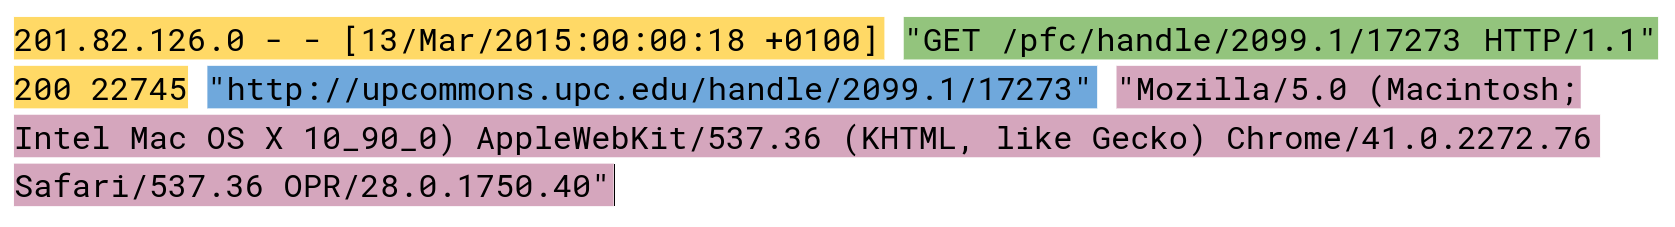
\includegraphics[width=1\textwidth]{figures/example-log}}
    \captionsetup{justification=centering}
    \caption[Exemple del contingut d'un \textit{\gls{log}}.]{Exemple del contingut d'un \textit{\gls{log}}. (\textbf{Font}: \gls{UPCommons}.)}\label{fig:example-log}
\end{figure}

\noindent
Cada línia present als fitxers dels \textit{\gls{log}s} correspon a una petició \gls{HTTP}.
El format d'aquesta és el següent:

\noindent \\
\textbf{Adreça \gls{IP}} \\ \\
Identificador de xarxa que indica l'agent que ha realitzat la petició.
L'agent pot ser:
\begin{itemize}
    \item Un usuari humà.
    \item Un agent automatitzat: robots, scripts, serveis de mail, etc. \\
\end{itemize}

\begin{tcolorbox}[colback=green!5!white, colframe=green!50!black, title=Els usuaris poden estar darrere d'un NAT]\label{tcbox:iguals-emmascarats}
    No podem sempre afirmar que dues peticions amb el mateix identificador provenen del mateix usuari.
    Pot haver-hi darrere un \gls{NAT}, usuaris compartint dispositiu, etc.
\end{tcolorbox}

\noindent \\
A causa de qüestions de privacitat i protecció de dades, aquest identificador ha sigut modificat en un procés d'anonimització.
Trobareu més informació respecte a aquest procés a l'annex~\ref{ch:log-anonymization}. \\

\clearpage

\noindent \\
\textbf{Data i hora} \\ \\
La marca temporal del registre ve definida per la seva data i hora.
Si bé es pot treballar directament amb aquest valor si segueix el format \gls{ISO}, és preferible utilitzar el format estàndard \gls{POSIX} (nombre de segons no intercalars des de l'1 de gener del 1970).
Aquest format és més simple, les comparacions són més eficients i evitem problemàtiques de diferències temporals en zones geogràfiques.

\noindent \\
\textbf{Informació de la petició \gls{HTTP}}~\cite{http} \\

\begin{itemize}
    \item Mètode de la petició: els més habituals són \texttt{GET}, \texttt{POST} i \texttt{HEAD}.
    \item Recurs accedit: enllaç al recurs accedit per la petició.
    \item Versió \gls{HTTP}: evolució d'\texttt{HTTP/1.0} fins a \texttt{HTTP/1.1} en el transcurs dels anys.
    No hi ha presència de registres amb \texttt{HTTP/2.0}.
    \item Codi d'estat que retorna la petició: codi que representa el resultat de la petició.
    Els més habituals són els \texttt{2XX} (succés), \texttt{3XX} (redireccions) \texttt{4XX} (error del client) i \texttt{5XX} (error del servidor)
    \item Mida de la resposta: mida en \textit{bytes} del cos de la resposta.
\end{itemize}

\noindent \\
\textbf{Referent} \\ \\
El camp del referent indica la ubicació d’on s’ha fet la sol·licitud del recurs accedit.

\noindent \\ \\
\textbf{User Agent} \\ \\
Amb l’ajuda d’aquest camp, podrem analitzar l’empremta digital del cercador utilitzat i determinar amb una certa precisió el tipus de dispositiu utilitzat, el sistema operatiu, si l’acció prové d’un usuari o d’una eina automatitzada (\textit{bots} o serveis de correu).

\clearpage

\subsection{Filtratge dels \textit{\gls{log}s}}\label{subsec:log-filter}

Un cop entenem l'estructura dels \textit{logs}, el següent pas és dur a terme un anàlisi preliminar del seu contingut.
Esmentarem diferents casos trobats durant el processament d'aquests. \\

\noindent
El cas principal, com hem vist a la figura~\ref{fig:example-log}, és aquell \textit{\gls{log}} que incorpora informació sobre un accés a un recurs, o una cerca.
Els podrem identificar perquè:

\begin{itemize}
    \item Porten l’identificador \gls{handle}.
    \item Contenen referències a algun domini d’\gls{UPCommons}.
    \item En cas ser una cerca a la plataforma, porten l’etiqueta amb alguna paraula clau com \textit{discover}, \textit{browse} \dots
\end{itemize}

\noindent
Però els servidors registren \textbf{moltes} més coses.
A continuació llistarem diversos casos identificats i la decisió presa en el seu processament.

\begin{itemize}
    \item Accés a recursos web.
    \item Repeticions.
    \item Cerques.
    \item Errors de processament.
\end{itemize}

\noindent \\
\textbf{Accés a recursos web} \\ \\
Després d’un accés a algun recurs, generalment als \textit{\gls{log}s} es poden veure registres d’accessos a recursos web (a la figura~\ref{fig:log-web-resource}, en vermell),
com podrien ser fitxers \textit{css}, \textit{javascript}, \textit{gifs} \dots

\begin{figure}[htbp]
    \centerline{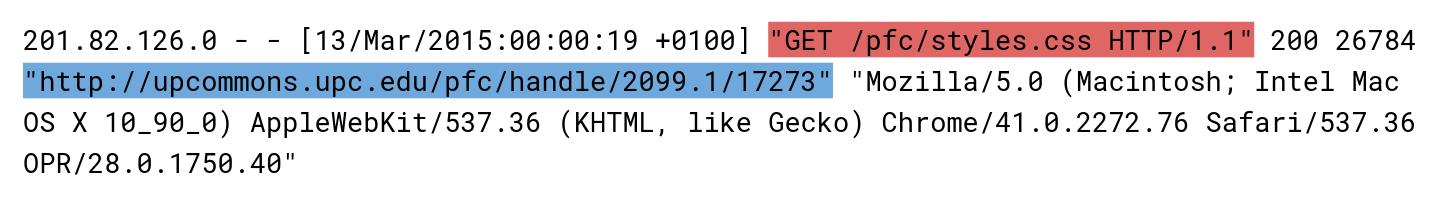
\includegraphics[width=\textwidth]{figures/log-web-resource}}
    \captionsetup{justification=centering}
    \caption[Exemple d'un \textit{\gls{log}} que accedeix a un recurs web, concretament una fulla d'estils \textit{\gls{CSS}}.]{Exemple d'un \textit{\gls{log}} que accedeix a un recurs web, concretament una fulla d'estils \textit{\gls{CSS}}. (\textbf{Font}: \gls{UPCommons}.)}\label{fig:log-web-resource}
\end{figure}

\noindent \\
Com que aquests registres no ens aporten cap informació valuosa pels nostres casos d'ús, els \textbf{descartarem}.

\clearpage

\noindent
\textbf{Repeticions} \\

\noindent
Un \textit{\gls{log}} apareix exactament igual a diverses entrades, amb una petita diferència temporal.
A la figura~\ref{fig:log-repetitions} podem veure com el mateix accés es repeteix tres vegades (verd i groc), a diferents adreces \gls{IP} (vermell).

\begin{figure}[htbp]
    \centerline{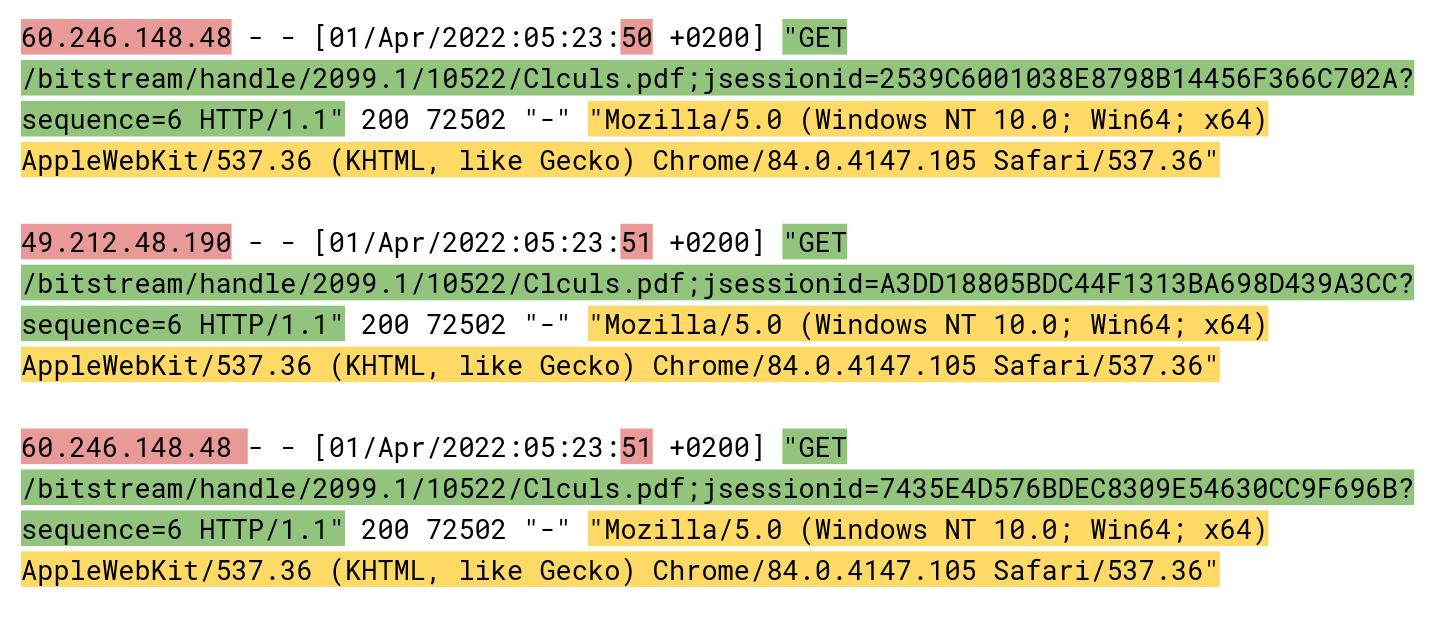
\includegraphics[width=\textwidth]{figures/log-repetitions}}
    \captionsetup{justification=centering}
    \caption[Exemple d'una cadena de \textit{\gls{log}s} que accedeixen al mateix contingut.]{Exemple d'una cadena de \textit{\gls{log}s} que accedeixen al mateix contingut. (\textbf{Font}: \gls{UPCommons}.)}\label{fig:log-repetitions}
\end{figure}

\begin{tcolorbox}[colback=green!5!white, colframe=green!50!black, title=Divergència relativa]
    No podem sempre afirmar que peticions amb contingut igual, però diferents identificadors provenen d'usuaris diferents.
    Pot haver-hi darrere un servidor \textit{Proxy} que redirigeixi les peticions, distribuïdors de càrrega, etc.
\end{tcolorbox}

\noindent
\begin{tcolorbox}[colback=blue!5!white, colframe=blue!75!black, title=Counter]
    Com a línia de treball futur, el projecte Counter~\cite{counter} pot servir com a base per tractar aquesta casuística.
\end{tcolorbox}

\noindent \\
Amb la finalitat d'enfocar l'anàlisi per altres bandes, no s'ha pres cap decisió en vers aquests casos, i seran tractats com la generalitat.

\clearpage

\noindent
\textbf{Cerques} \\

\noindent
Als \textit{\gls{log}s} hi són presents cerques dins de la plataforma \gls{UPCommons}.
Detectem aquests casos ja que la comanda és una paraula clau de cerca.
A l'exemple de la figura~\ref{fig:log-search} s'utilitza \textit{browse}, però n'hi ha d'altres com \textit{discover}, \textit{search} \dots \\

\begin{figure}[htbp]
    \centerline{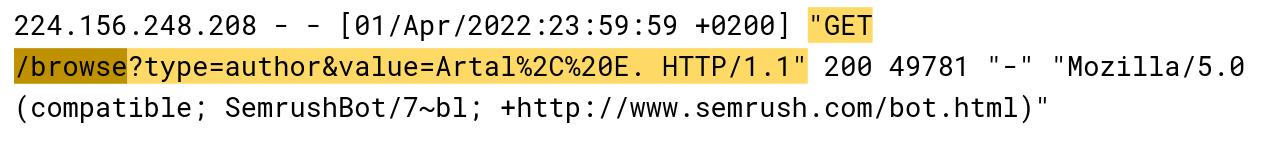
\includegraphics[width=\textwidth]{figures/log-search}}
    \captionsetup{justification=centering}
    \caption[Exemple d'un \textit{\gls{log}} d'una cerca a la plataforma.]{Exemple d'un \textit{\gls{log}} d'una cerca a la plataforma. (\textbf{Font}: \gls{UPCommons}.)}\label{fig:log-search}
\end{figure}

\noindent
El procediment general no canvia respecte a aquest cas.
Haurem de tenir en compte quins són, i diferenciar-los de la resta. \\

\noindent
\textbf{Errors de processament}\label{subsubsection:log-errors} \\

\noindent
Diem que un \textit{\gls{log}} produeix un error de processament si el seu format difereix abruptament del general (vegeu ~\ref{subsec:log-analysis}).
Diferenciarem entre dos casos:

\begin{itemize}
    \item \textbf{Errors reversibles:} són aquells que segueixen un paradigma.
    La seva presència és abundant.
    Alguns exemples śon:
    \begin{itemize}
        \item L'adreça \gls{IP} no existeix o està mal formada.
        \item Contingut alterat (a vegades, intencionadament!)
    \end{itemize}
    En aquests casos manipularem el registre afectat per homogeneïtzar el conjunt dels \textit{logs}.
    \item \textbf{Errors irreversibles:} alteració en grau superlatiu del cos del \textit{log}.
    Dificulta el seu processament.
    La seva presència és escassa.
    El resultat d'afegir la lògica necessària per tractar aquests casos no justifica en cap cas el seu tractament.

    Per aquests motius, aquests casos es descartaran.
    El nombre total de registres descartats es troba documentat al Capítol~\ref{ch:log-storing}, a la taula~\ref{tab:logs-table}.
\end{itemize}

\noindent
\begin{tcolorbox}[colback=green!5!white, colframe=green!50!black, title=No val la pena]\label{tcbox:no-val-la-pena}
Parlem d'afegir condicions al processament que només s'utilitzarien en el 0,000000287\% dels casos.
\tcblower 552 \textit{\gls{log}s} de 1.922.392.760
\end{tcolorbox}

\clearpage

\subsection{Disseny tècnic}\label{subsec:logs-technical-design}

Un cop tenim el \textbf{què} sobre els \textit{\gls{log}s}, passem al \textbf{com} els processem.
L'objectiu és proposar una solució que abasti el procés que es durà a terme des de la lectura d’un \textit{\gls{log}} fins a la seva agregació a la base de dades. \\

\noindent
La nostra premissa és la següent:
\noindent
\begin{center}
    \texttt{DB.insert(transform(log, Y[])) if filter(log, X[])}
\end{center}

\noindent
Que es traduiria a:
\begin{center}
    Insereix a la base de dades el \textit{\gls{log}} que compleixi cert criteri i fes-ho amb aquest format.
\end{center}

\begin{figure}[htbp]
    \centerline{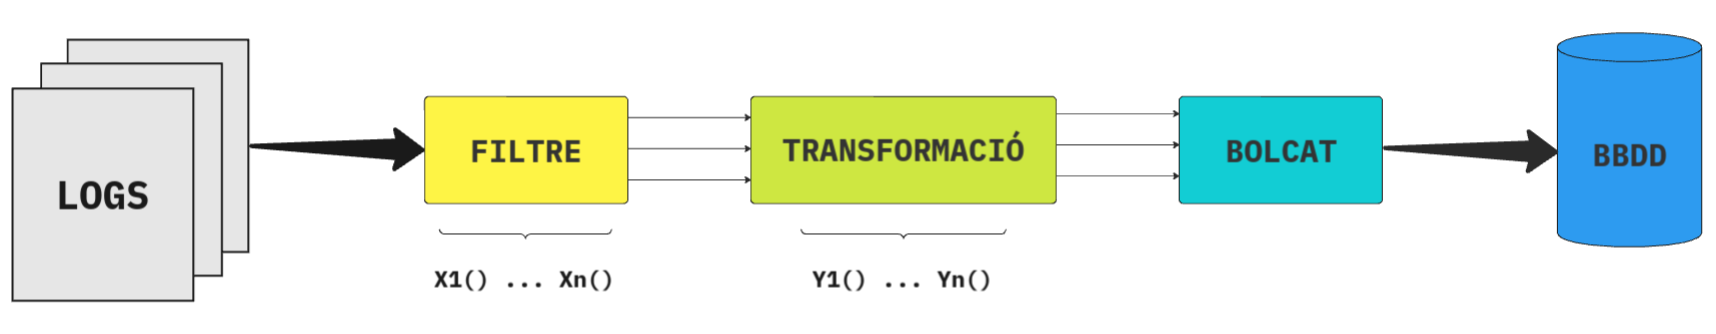
\includegraphics[width=1\textwidth]{figures/log-processing}}
    \captionsetup{justification=centering}
    \caption[Disseny tècnic del processament dels \textit{logs}.]{Disseny tècnic del processament dels \textit{logs}. (\textbf{Font}: Elaboració pròpia.)}\label{fig:log-processing}
\end{figure}

\noindent
El disseny proposat a la figura~\ref{fig:log-processing} té tres components principals: \\

\noindent
\textbf{Component \texttt{Filtre}} \\

\noindent
El component \texttt{Filtre} s’encarrega de filtrar cada \textit{\gls{log}} mitjançant un criteri específic.
Per exemple:
\begin{itemize}
    \item Si només volem admetre \textit{\gls{log}s} que provenen de dispositius mòbils, definirem una funció filtre que ho faci.
\end{itemize}

\noindent
Les funcions de \texttt{Filtre} poden ser additives, és a dir, un mateix \textit{\gls{log}} pot ser filtrat per diverses funcions.
Si cap filtre és necessari, no es definirà cap. \\

\clearpage

\noindent
\textbf{Component \texttt{Transformació}} \\

\noindent
L’objectiu del component \texttt{Transformació} és modificar el format del \textit{\gls{log}} per afegir o treure camps segons els criteris determinats.
Per exemple:

\begin{itemize}
    \item Podem definir una funció de transformació per canviar del format de la data i hora a un UNIX \textit{\gls{timestamp}}.
    \item Eliminar algun camp que es consideri irrellevant s’hauria de fer mitjançant funcions de transformació.
\end{itemize}

\noindent
Les funcions de \texttt{Transformació} poden ser additives, és a dir, un mateix \textit{\gls{log}} pot ser reformat per diverses funcions.
Si cap transformació és necessària, no es definirà cap. \\

\noindent
\textbf{Component \texttt{Bolcat}} \\

\noindent
Finalment, al component \texttt{Bolcat} arribarà el conjunt de \textit{\gls{log}s} desitjats amb el format escollit.
Ara bé, depenent de la base de dades on es vol fer l’agregació, és possible que s’hagin de fer petits retocs per compatibilitat amb la base de dades. \\

\noindent
\textbf{Processament}

\noindent \\
Així mateix, si tenim \(X_1\)..\(X_N\) funcions filtre, i \(Y_1\)..\(Y_N\) funcions de transformació, i dos casos d’ús, podem definir el comportament desitjat de la següent manera:

\begin{itemize}
    \item \textbf{Cas d'ús \#1}: processa tots els logs, canvia el format de la data i envia'ls a una base de dades PostgreSQL.
    \begin{itemize}
        \item \texttt{Filtre:} -
        \item \texttt{Transformació:} \(Y_1\)
        \item \texttt{Bolcat:} \texttt{PostgreSQLForwarder}
    \end{itemize}
    \item \textbf{Cas d'ús \#2}: processa només els \textit{\gls{log}s} que accedeixin a recursos UPC, afegeix l’enllaç permanent i guarda-ho a un fitxer pla:
    \begin{itemize}
        \item \texttt{Filtre:} \(X_2\)
        \item \texttt{Transformació:} \(Y_2\)
        \item \texttt{Bolcat:} \texttt{FileSystemForwarder}
    \end{itemize}
\end{itemize}

\noindent
Finalment, enviaríem al codi els casos d’ús: \(CU_1\), \(CU_2\) des d'un fitxer de configuració/codi que faci la feina.

\clearpage

\subsection{Implementació}\label{subsec:log-implementation}

\noindent
\texttt{Filtre}.
La interfície del mòdul filtre requereix que les seves implementacions disposin d'una funció \texttt{filter}.
\begin{center}
    \texttt{function filter(Log) -> bool}
\end{center}
Aquesta ha d'acceptar un \textit{\gls{log}} com a paràmetre explícit, i retornar cert, si i només si aquell registre passa el filtre definit.

\noindent \\
S'han desenvolupat les següents funcions:

\begin{itemize}
    \item \texttt{WebResource}: Detecta si el recurs accedit és un recurs web.
    \item \texttt{SearchResource}: Detecta si és una cerca d’un recurs.
    \item \texttt{AccessResource}: Detecta si el recurs accedit és un recurs d’\gls{UPCommons} a través de l'identificador \gls{handle}.
    \item \texttt{WithIPv6Address}: Detecta si el \textit{\gls{log}} té present l’adreça en versió IPv6.
    \item \texttt{WithoutIpAddress}: Detecta si el \textit{\gls{log}} no té present el camp d'adreça \gls{IP}.
    \item \texttt{AccessResourceBitstream}: Detecta si el recurs accedit és un recurs d’UPCom-mons a través de l'identificador \gls{bitstream} \gls{UUID}.
\end{itemize}

\noindent \\
\texttt{Bolcat}:
\begin{itemize}
    \item \texttt{InfluxDbForwarder}:
    \begin{itemize}
        \item Adapta el \textit{\gls{log}} en format JSON al format específic de la base de dades.
        \item Envia el \textit{\gls{log}} a la base de dades.
    \end{itemize}
\end{itemize}

\clearpage

\noindent
\texttt{Transformació}.
La interfície del mòdul filtre requereix que les seves implementacions disposin d'una funció \texttt{transform}.
A causa de la variabilitat d'aquestes funcions, la interfície no exigeix en forma de contracte cap funció.

\noindent \\
S'han desenvolupat les següents funcions:

\noindent \\
\texttt{Transformació}:
\begin{itemize}
    \item \texttt{ToJSON}: Converteix un \textit{\gls{log}} emmagatzemat en una seqüència de caràcters en un \gls{JSON} estructurat.
    \item \texttt{AddLabel}: Afegeix al JSON un parell clau valor.
    \item \texttt{AddTimestamp}: Extrau i afegeix el valor de la data i l'hora.
    \item \texttt{RemoveIPv6Address}: Elimina la adreça \gls{IP} en format IPv6 i manté aquella en format IPv4.
    \item \texttt{AddResourceIdLabel}: Afegeix l'identificador del recurs al qual accedeix el \textit{log}, en cas que aquest sigui un accés a un recurs.
    \item \texttt{AddDefaultIpAddress}: Afegeix una adreça \gls{IP} constant a aquells \textit{\gls{log}s} que no en tinguin cap.
\end{itemize}

\noindent
Un cop definides les funcions individualment, el procés global per processar els \textit{\gls{log}s} es descriu amb el diagrama de la figura~\ref{fig:log-processing-workflow}.

\noindent
\begin{figure}[htbp]
    \centerline{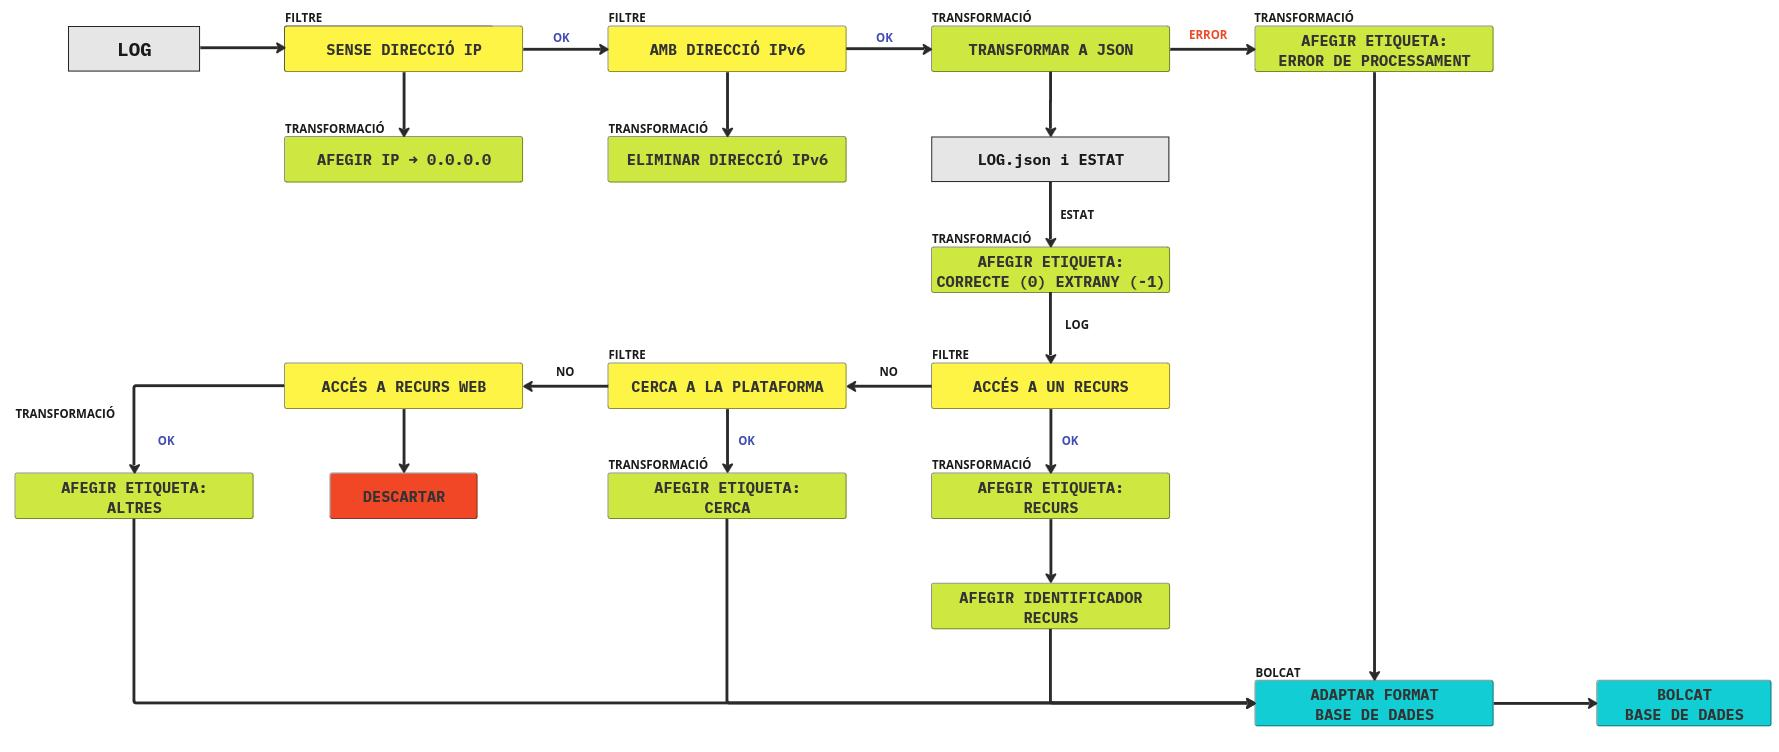
\includegraphics[width=1.1\textwidth]{figures/log-processing-workflow}}
    \captionsetup{justification=centering}
    \caption[Implementació del processament dels \textit{logs}.]{Implementació del processament dels \textit{logs}. (\textbf{Font}: Elaboració pròpia.)}\label{fig:log-processing-workflow}
\end{figure}
\clearpage
\section{Metadades}\label{sec:metadata-processing}

Les metadades són el conjunt d'etiquetes presents als registres d'\gls{UPCommons} que contenen informació sobre aquest.
Els autors, la descripció del recurs, la data de pujada, el departament responsable, el tipus de document, o més, es troben inclosos. \\

\noindent
En el nostre cas, a \gls{UPCommons}, aquestes utilitzen el format \gls{DSpace} Intermediate Metadata, \gls{DIM}.
Es basa a fer servir el format Dublin Core incorporant un qualificador, amb la finalitat d'afinar la informació que .
L'estructura és la següent:

\begin{center}
    \textit{schema.element.qualifier} \\
\end{center}

\noindent
Per exemple, l'autor principal d'un recurs s'identificaria com:

\begin{center}
    \text{dc.contributor.author} \\
\end{center}

\noindent
Per cada metadada, s'assignen els següents valors:

\begin{itemize}
    \item \textbf{value}: Valor de la metadada.
    \item \textbf{language}: Idioma.
    És habitual trobar-lo a les descripcions / resums dels registres, encara que a vegades no està ben introduït.
    \item \textbf{authority}: Codi que relaciona la metadada amb un sistema d'autoritats que permet obtenir més dades.
    \item \textbf{qualifier}: Un nivell de confiança associat a l'autoritat.
\end{itemize}

\clearpage

\noindent
A continuació es mostren algunes metadades extretes d'un recurs, on es pot contemplar tant el format de les metadades, com els valors. \\

\begin{tcolorbox}[colback=green!5!white, colframe=green!50!black, title=Metadades]
    Al web només hi apareix el \textbf{\textit{value}} o el \textbf{\textit{language}} de la metadada, els altres camps s'emmagatzemen internament.
\end{tcolorbox}

\begin{figure}[htbp]
    \centerline{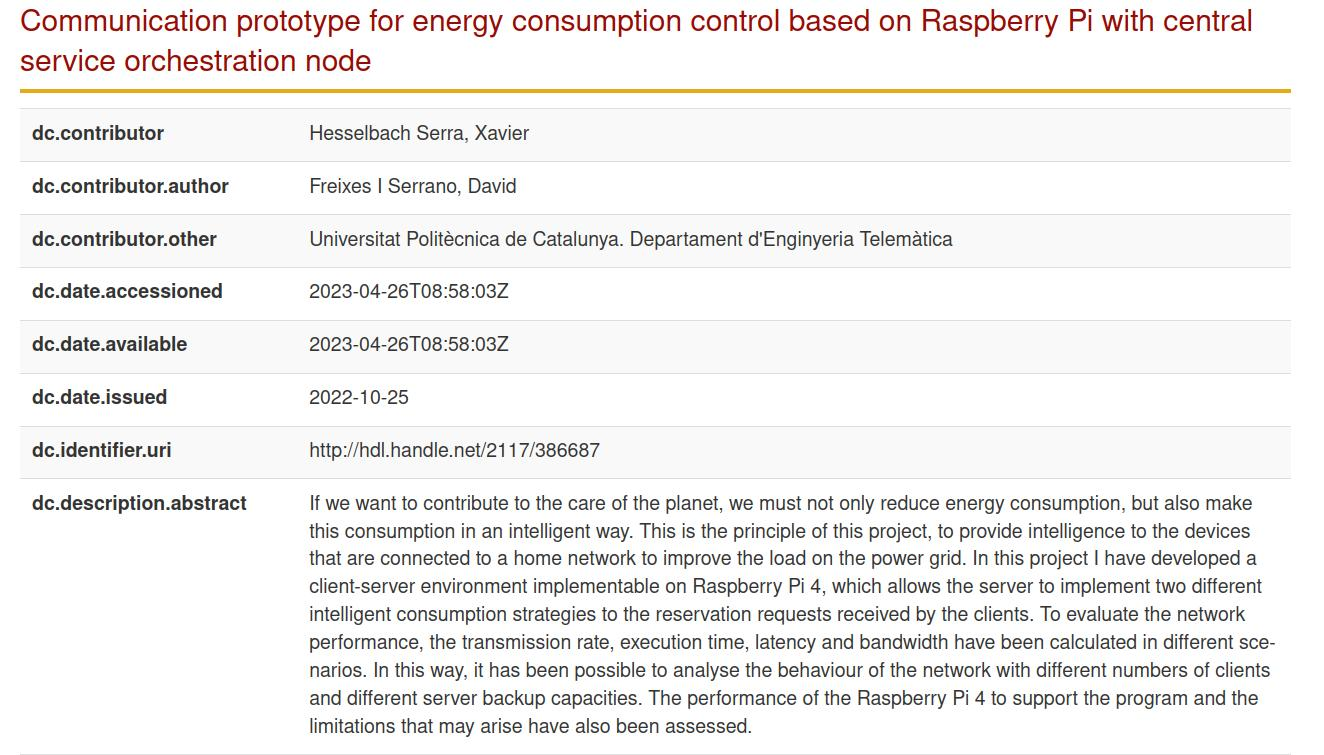
\includegraphics[width=\textwidth]{figures/metadata-example}}
    \captionsetup{justification=centering}
    \caption{Llista parcial de les metadades d'un recurs. (\textbf{Font}: \url{http://hdl.handle.net/2117/386687})}\label{fig:metadata-example}
\end{figure}

\clearpage

\subsection{\gls{OAI-PMH}}\label{subsec:oai-pmh}

El protocol \gls{OAI-PMH} (Open Archive Initiative-Protocol for Metadata Harvesting) és un estàndard d'interoperabilitat desenvolupat per l'intercanvi i la difusió de metadades. \\

\noindent
Permet accedir a metadades codificades en diferents formats, encara que el més habitual és el Dublin Core. \\

\noindent
Aquest protocol defineix sis operacions bàsiques~\cite{oai-pmh}:

\begin{itemize}
    \item \textbf{\texttt{GetRecord}}: utilitzat per obtenir informació sobre un registre individual.
    \item \texttt{\textbf{Identify}}: emprat per aconseguir informació sobre el repositori.
    \item \texttt{\textbf{ListIdentifiers}}: retorna les capçaleres dels registres.
    \item \texttt{\textbf{ListMetadataFormats}}: retorna els formats de metadades disponibles al repositori.
    \item \texttt{\textbf{ListRecords}}: verb principal per la recol·lecta de metadades, retorna els registres complets.
    \item \texttt{\textbf{ListSets}}: retorna l’estructura dels \textit{sets} del repositori.
\end{itemize}

\clearpage

\subsection{Control de Flux}\label{subsec:flux-control}

Alguns servidors implementen un mecanisme de control de flux per tal de tractar les peticions que retornin llistes incompletes.
Es basa a utilitzar un identificador anomenat \textit{resumptionToken}, que retorni la petició anterior amb la llista incompleta, i sigui paràmetre de la següent petició. \\

\begin{tcolorbox}[colback=blue!5!white, colframe=blue!75!black, title=Finestra lliscant]
    Per comparar-ho amb altres protocols, \gls{TCP}~\cite{tcp} utilitza el valor de la ``finestra lliscant'' per indicar la quantitat de dades que ha d'enviar l'emissor,
    i per \textbf{on} ha de començar, ja que aquest valor es suma al número de seqüència.
\end{tcolorbox}

\noindent \\
El procés s'iterarà fins a obtenir la llista completa.
Podrem identificar el final, pel fet que:

\begin{itemize}
    \item Aquesta darrera llista té una grandària inferior a les anteriors (acostuma a ser 100 unitats).
    \item El valor del \textit{resumptionToken} és nul. \\
\end{itemize}

\noindent
L'objectiu és, altrament que la fragmentació de peticions que demanen quantitats ciclòpiques de dades és més operatiu,
permet la recuperació del context en cas d'errors de xarxa o d'altra classe.

\clearpage

\subsection{Implementació}\label{subsec:metadata-implemntation}

L'objectiu és clar, descarregar totes les metadades.
El protocol està ben definit.
La llibreria Sickle~\cite{Sickle} ens facilita la feina.
Això resulta en una implementació senzilla:

\begin{enumerate}
    \item Connectar-se al servidor \gls{OAI} .
    \item Demanem les metadades:
    \begin{enumerate}
        \item Disposem de la llista (incompleta) de registres de metadades.
        \item Extraiem aquella informació rellevant pel nostre cas d'ús, que són les metadades en format Dublin Core.
        \item Descartem aquells registres marcats com esborrats, ja que no contenen cap informació.
        \item Realitzem l'abocament a la base de dades corresponent.
    \end{enumerate}
    \item Tornem a iterar fins a obtenir la llista completa de les metadades.
\end{enumerate}

\begin{figure}[htbp]
    \centerline{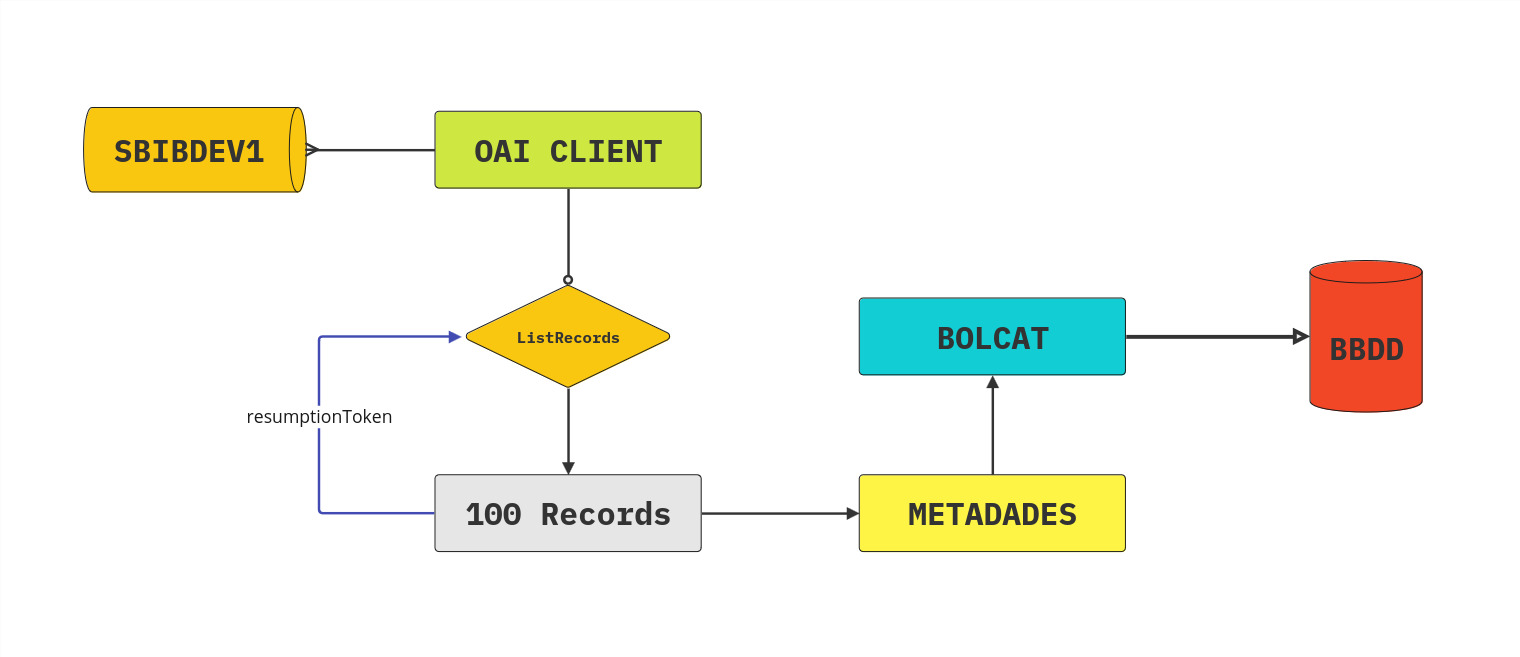
\includegraphics[width=1.2\textwidth]{figures/metadata-processing}}
    \captionsetup{justification=centering}
    \caption{Disseny tècnic del processament de les metadades. (\textbf{Font}: Elaboració pròpia.)}\label{fig:log-analysis}
\end{figure}


\chapter{Emmagatzematge de les dades}\label{ch:log-storing}

L’objectiu principal de l’ús de bases de dades és de disposar d’una eina que ens permeti efectuar operacions com la cerca, indexació i emmagatzemament dels logs.
Treballar directament sobre arxius plans no és gens recomanable.

\clearpage
\section{Logs}\label{sec:logs-storing}

El següent conjunt de paràmetres és el que permet agrupar tota la informació present als \textit{\gls{log}s}.
L’evolució al llarg dels anys no ha afectat gaire respecte als paràmetres existents sinó al contingut d’aquests. \\

\noindent
Aquí un exemple d’un \textit{log}:

\begin{itemize}
    \item \texttt{ip\_address:  39.92.248.6}
    \item \texttt{date: 20/Apr/2011}
    \item \texttt{time: 23:59:59 +0200}
    \item \texttt{request}:
    \begin{itemize}
        \item \texttt{method: GET}
        \item \texttt{resource: /e-prints/bitstream/2117/8469/1/sdarticle.pdf}
        \item \texttt{version: HTTP/1.0}
        \item \texttt{status\_code: 304}
        \item \texttt{response\_size: -}
    \end{itemize}
    \item \texttt{referer: null}
    \item \texttt{user\_agent:  gsa-crawler (Enterprise; T2-QGG2U8NZXNSAA upcnet\\.backoffice.aps@upcnet.es)}
\end{itemize}


\noindent \\
Aquesta estructura de dades representa la informació que podem extreure directament dels \textit{\gls{log}s} provinents d'\gls{UPCommons}.
El resultat del nostre processament d'aquests altera aquest format per afegir més informació, com veurem més endavant.

\clearpage

\subsection{Bases de dades candidates}\label{subsec:log-db-options}

\noindent \\
A continuació llistarem les opcions candidates a ser el sistema gestor de bases de dades on emmagatzemarem tots els logs.

\noindent \\
La majoria són sistemes d’agregació de logs, que incorporen eines de monitoratge, sistemes d’alertes, visualització, etc.
És criteri nostre fer-ne ús d’aquests serveis o només continuar amb la base de dades.

\noindent \\
Com a primeres opcions considerem aquelles que siguin de programari lliure i en les quals puguem instal·lar localment la base de dades.

\noindent \\
\textbf{Grafana Loki~\cite{loki:main}}\label{subsubsec:log-db-option-loki}

\noindent \\
\textit{Grafana Labs} proporciona \textit{Loki}, un sistema d’agregació de \textit{\gls{log}s} de codi obert, basat en Prometheus.
És un sistema distribuït i dissenyat per ser escalable.
Les seves característiques principals són:

\begin{itemize}
    \item \textbf{Escalabilitat}: Disposa de diferents modes de desplegament on pots escollir el que més s’adapti als teus requisits.
    \item \textbf{Integració}: Suporta diverses implementacions/llibreries de tercers per fer-ne servir, i diversos modes de desplegament en local.
    \item \textbf{Grafana}: Integració per defecte amb \textit{Grafana} com a eina principal d’observabilitat.
    \item \textbf{Emmagatzemament}: Loki només indexa les metadades dels \textit{\gls{log}s}~\cite{loki:indexing}, és a dir, només el \textit{\gls{timestamp}} i els \textit{labels} definits.
    El contingut del \textit{\gls{log}} no s’indexa.
    Utilitzant aquest plantejament, s’aconsegueix reduir la quantitat total d'espai de disc necessari.
    \begin{itemize}
        \item Aquesta característica és bastant interessant si utilitzem aquests \textit{labels} per afegir informació relacionada amb el recurs accedit per a després com a millorar el procés de cerca.
    \end{itemize}
\end{itemize}

\clearpage

\noindent
\textbf{Elastic~\cite{elastic}}

\noindent \\
Elastic, conegut pel seu motor de cerca Elasticsearch, disposa d’una solució de monitoratge de \textit{\gls{log}s}.
Les seves característiques principals:

\begin{itemize}
    \item \textbf{Escalabilitat}: dissenyat per monitorar \textit{\gls{log}s} fins a una escala de \textit{petabytes}.
    \item \textbf{Integració}: suporta diverses implementacions/llibreries de tercers per fer-ne servir, i modes de desplegament en local.
    \item \textbf{\textit{Logstash}}: mecanisme per centralitzar i transformar les dades per a després emmagatzemar-les a qualsevol lloc.
    \item \textbf{\textit{Kibana}}: integració per defecte amb \textit{Elastic Kibana} com a eina principal d’observabilitat.
    \item \textbf{Categorització}: incorpora una eina per identificar patrons, tendències i anomalies als \textit{\gls{log}s}.
\end{itemize}


\noindent \\
\textbf{Apache SOLR~\cite{SOLR}}

\noindent \\
Apache SOLR és una plataforma de cerca que es pot utilitzar com a mecanisme d’emmagatzemament de documents. 
Les seves característiques principals:

\begin{itemize}
    \item \textbf{Escalabilitat}: basat en un sistema distribuït i rèpliques, és optimitzat per grans volums de dades.
    \item \textbf{Integració}: la comunicació amb el servei es realitza mitjançant l’\gls{API} de SOLR sobre \gls{HTTP} .
    També suporta diferents modes de desplegament en local.
    \item \textbf{Lucene}: fa servir \textit{Apache Lucene} com a motor de cerca principal.
\end{itemize}

\noindent
Com a contrapartida:

\begin{itemize}
    \item \textbf{Visualització}: no disposa d’un sistema de visualització de dades per defecte, així perque caldria emprar-ne un de tercers.
\end{itemize}


\clearpage

\noindent
Altres opcions que no són de codi obert, la versió gratuïta que proporcionen és bastant limitada o no hi ha prou documentació a la xarxa són les següents:

\begin{itemize}
    \item \textbf{Graylog}~\cite{graylog}
    \item \textbf{Papertrail}~\cite{papertrail}
    \item \textbf{Loggly}~\cite{loggly}
    \item \textbf{Splunk}~\cite{splunk}
\end{itemize}

\noindent \\
\subsection{Decisió}\label{subsec:log-db-decision}

\noindent
La primera decisió presa fou donar suport a \textit{Grafana Loki}, amb els motius que llistarem a continuació:

\begin{itemize}
    \item Base de dades de codi obert compatible per diferents plataformes.
    \item És una eina ben documentada~\cite{loki:documentation}.
    \item Té una gran quantitat d’usuaris actius.
    El repositori de codi~\cite{loki:code} és mantingut activament i de forma actual.
    \item Integració per defecte amb \textit{Grafana} per poder visualitzar els \textit{logs}.
    \item Diverses llibreries~\cite{loki:libraries} ja implementades per enviar \textit{\gls{log}s} a la base de dades.
    \item Com prèviament s’ha mencionat, la indexació és a partir del \textit{\gls{timestamp}} més les metadades.
    Aquestes darreres poden ser utilitzades per afegir valors que després agilitzaran el processament. \\
\end{itemize}

\noindent
Com podem veure a la imatge~\ref{fig:loki-indexing}, converteixen un \textit{\gls{log}} semblant als nostres en un altre adaptat al format de loki, on utilitzen com etiqueta el tipus petició (\textit{action}) o el codi d’estat (\textit{status\_code}) \\ \\
El nostre cas, en podem afegir uns que indiquin el tipus de \textit{\gls{log}} (cerca, accés a recurs) o marcar-ne alguns que tinguin algun contingut inexacte.

\clearpage

\begin{figure}[htbp]
    \centerline{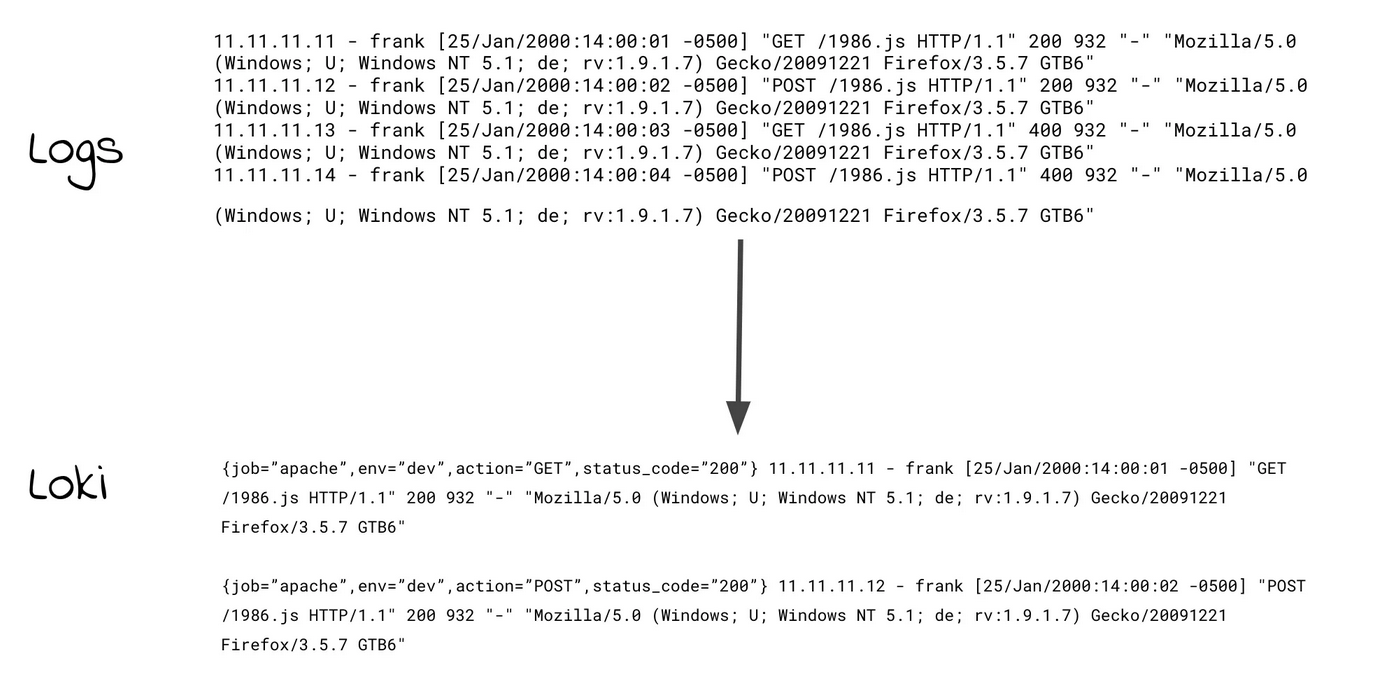
\includegraphics[width=1\textwidth]{figures/loki-indexing}}
    \captionsetup{justification=centering}
    \caption[Exemple del funcionament de la indexació dels paràmetres a \textit{Grafana Loki}.]{Exemple del funcionament de la indexació dels paràmetres a \textit{Grafana Loki}. (\textbf{Font}: \url{https://medium.com/geekculture/pushing-logs-to-loki-without-using-promtail-fc31dfdde3c6})}\label{fig:loki-indexing}
\end{figure}

\noindent \\
Malauradament, errors durant l’etapa de configuració, concretament del paràmetre que defineix el temps màxim d'anterioritat per la cerca dels \textit{\gls{log}s}, ens van fer recular i considerar altres opcions.

\clearpage

\noindent
La següent opció és \textit{InfluxDb}.
Aquesta base de dades, també basada en series temporals, té característiques similars a l’anterior:

\begin{itemize}
    \item Base de dades de codi obert compatible per diferents plataformes.
    \item És una eina ben documentada~\cite{influxdb:documentation}.
    \item Té una gran quantitat d’usuaris actius.
    El repositori de codi~\cite{influxdb:code} és mantingut activament i de forma actual.
    \item Integració per defecte amb Grafana per poder visualitzar els \textit{logs}.
    \begin{itemize}
        \item Aquest és un dels punts que ens van fer considerar aquesta opció, ja que va ser recomanada pel mateix aplicatiu de Grafana.
    \end{itemize}
    \item Diverses llibreries~\cite{influxdb:libraries} ja implementades per enviar \textit{\gls{log}s} a la base de dades.
    \begin{itemize}
        \item En el nostre cas emprar \textit{influxdb-client}~\cite{influxdb:python} pel llenguatge \textit{Python}.
    \end{itemize}
    \item En aquest cas, però, la indexació és a partir dels \textit{tags} (``tag set'' a la figura~\ref{fig:loki-indexing}).
    Utilitzarem aquest camp per afegir valors freqüents, que poden ser agrupats i fàcilment indexats.
\end{itemize}

\begin{figure}[htbp]
    \centerline{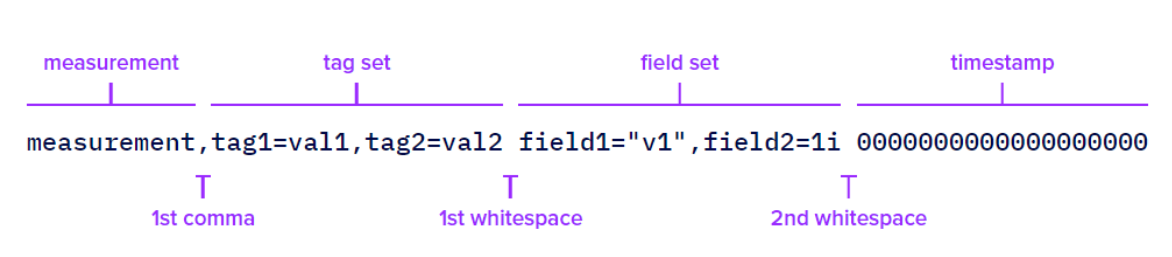
\includegraphics[width=1\textwidth]{figures/influxdb-indexing}}
    \captionsetup{justification=centering}
    \caption[Exemple del funcionament de la indexació dels paràmetres a \textit{InfluxDb}.]{Exemple del funcionament de la indexació dels paràmetres a \textit{InfluxDb}. (\textbf{Font:} \url{https://docs.influxdata.com/influxdb/v2/get-started/write/\#line-protocol-element-parsing})}\label{fig:influxdb-indexing}
\end{figure}

\clearpage

\subsection{Procés d'abocament dels \textit{\gls{log}s}}\label{subsec:log-push}

\noindent
El procés d’abocament dels \textit{\gls{log}s} consisteix a migrar tots els \textit{\gls{log}s} d’una estructura de fitxers, emmagatzemats en un directori, a un sistema gestor de bases de dades. \\

\noindent
Els \textit{\gls{log}s} es trobaven emmagatzemats a \texttt{/mnt/working/logsanon}, on hi havia un fitxer comprimit amb tots els registres per cada dia. \\

\noindent
Per tal de poder fragmentar la tasca, s’ha desenvolupat un petit \textit{script} que descomprimeixi aquests arxius, i el més important, seguint aquesta estructura de fitxers com a ubicació destí:

\begin{verbatim}
    2006
    |-- 01
    |   |-- 2006-01-01.log
    |   |-- ...
\end{verbatim}
\noindent
D’aquesta manera, podem realitzar l’abocament de manera esglaonada (any per any, mes a mes, etc.) i acotada.

\noindent \\
La base de dades escollida, com prèviament s’ha documentat (veure~\ref{subsec:log-db-decision}), és \textbf{InfluxDb}.
Per tal de poder enviar les dades, hem fet ús de la llibreria oficial~\cite{influxdb:python} que ofereix la plataforma pel llenguatge Python.

\clearpage

\noindent
\textbf{Format de les dades} \\ \\
\textbf{InfluxDb} emmagatzema les dades utilitzant el que anomenen el ``Line protocol''.
Esquematitzant-ho, i amb el suport de la figura~\ref{fig:influxdb-indexing}, tractarem quatre paràmetres:

\begin{itemize}
    \item \texttt{measurement}: identificador principal de les dades.
    \item \texttt{tag set}: conjunt de parelles clau-valor \textbf{indexades}.
    Farem ús d'aquest camp per afegir valors freqüents, que poden ser agrupats i fàcilment indexats:
    \begin{itemize}
        \item \textbf{content}: format del contingut, pot ser:
        \begin{itemize}
            \item \texttt{ok}: el format del \textit{\gls{log}} és l'esperat.
            \item \texttt{diferent}: el format del \textit{\gls{log}} no és l'esperat però s'ha pogut tractar.
            \item \texttt{error}: error de processament.
        \end{itemize}
        Vegeu errors de processament~\ref{subsubsection:log-errors}.
        \item \textbf{method}: mètode \gls{HTTP} present al \textit{\gls{log}}.
        \item \textbf{status\_code}: codi d'estat de la resposta de la petició d'\gls{HTTP} .
        \item \textbf{type}: tipus de \textit{\gls{log}}, pot ser:
        \begin{itemize}
            \item \texttt{cerca}: cerca a la plataforma d'\gls{UPCommons}.
            \item \texttt{recurs}: accés a un recurs d'\gls{UPCommons}.
            \item \texttt{altres}: altres tipus de \textit{\gls{log}}.
        \end{itemize}
        Vegeu filtrage dels \textit{\gls{log}s}~\ref{subsec:log-filter}.
    \end{itemize}
    \item \texttt{field set}: conjunt de parelles clau-valor \textbf{no indexades}.
    Aquí hi emmagatzemarem valors únics, com són:
    \begin{itemize}
        \item \textbf{log}: registre complet d'\gls{UPCommons}.
        \item \textbf{recurs}: identificador \gls{handle}, en cas que es tracti d'un accés a un recurs.
    \end{itemize}
    \item \texttt{\gls{timestamp}}: marca temporal en nanosegons.
\end{itemize}

\clearpage

\noindent
\textbf{Optimitzacions} \\ \\

\noindent
La implementació del client d'InfluxDb ha estat optimitzada~\cite{influxdb:optimizations} de la següent manera:

\begin{itemize}
    \item \texttt{batching}: El mode d'escriptura emprat és el \textit{batching}.
    Consisteix a agrupar els elements (\textit{\gls{log}s}) en tandes, i després enviar una petició d'escriptura.
    A causa del volum de dades que tractem, evitem enviar una petició per cada \textit{log}, alleugerint la càrrega computacional.
    \begin{tcolorbox}[colback=red!5!white, colframe=red!75!black, title=Sobrecàrrega]
    En cas de disposar de la base de dades en algun servei de \textit{cloud}, aquest problema s'agreujaria, incrementant la latència.
    \end{tcolorbox}
    \item \texttt{flush\_interval}: La mida de les tandes (\textit{batches}) és de 500 elements.
    A part d’això, establim una marca temporal mínima en què s’envien les dades.
    És a dir, enviem una petició d’escriptura si es compleix alguna de les següents condicions:
    \begin{itemize}
        \item S’ha arribat a la mida del \textit{batch}: 500.
        \item Ha passat dos segons des de la darrera petició d’escriptura.
    \end{itemize}
    \item \texttt{tags}: El diccionari que conté les etiquetes amb informació rellevant del \textit{\gls{log}} s’ha ordenat alfabèticament a partir de les claus.
    \item \texttt{\gls{timestamp}}: Enviem el \textit{\gls{log}} amb la marca temporal amb precisió de l’orde dels nanosegons, format que utilitza \textbf{InfluxDb}.
    \item \texttt{\gls{gzip}}: comprimint les dades podem accelerar el procés d’escriptura fins a cinc vegades, tal com indica la guia d'optimització d'InfluxDb~\cite{influxdb:optimizations}
\end{itemize}

\clearpage

\noindent
\textbf{Estadístiques} \\ \\

\noindent
El resultat de l’abocament conclou amb la següent taula on es mostren alguns números interessants. \\ \\
Podeu consultar els resultats parcials, dividits per any a l'Annex~\ref{ch:log-push-results}. \\

\begin{table}[h!]
    \centering
    \begin{adjustbox}{width=1.2\textwidth, center}
        \begin{tabular}{|l|r|r|r|r|r|r|r|}
            \toprule
            \begin{tabular}[c]{@{}l@{}}   \textbf{Any}                                                      \end{tabular}
            & \begin{tabular}[c]{@{}l@{}} \textbf{Nº total} \\ \textbf{de logs}                             \end{tabular}
            & \begin{tabular}[c]{@{}l@{}} \textbf{Accés a recursos} \\ \textbf{UPCcommons}                  \end{tabular}
            & \begin{tabular}[c]{@{}l@{}} \textbf{Cerques a} \\ \textbf{UPCcommons}                         \end{tabular}
            & \begin{tabular}[c]{@{}l@{}} \textbf{Accés a recursos} \\ \textbf{web descartats}              \end{tabular}
            & \begin{tabular}[c]{@{}l@{}} \textbf{Altres tipus} \\ \textbf{de logs}                         \end{tabular}
            & \begin{tabular}[c]{@{}l@{}} \textbf{Errors de} \\ \textbf{processament}                       \end{tabular}
            & \begin{tabular}[c]{@{}l@{}} \textbf{Duració de} \\ \textbf{l'abocament} \\ \textbf{(minuts)}  \end{tabular}   \\
            \midrule
            \textbf{2006}       & 1.553.768             & 239.410               & 584.614                   & 325.932               & 405.372                   & 155           & 1,62          \\
            \textbf{2007}       & 15.052.731            & 3.039.294             & 2.043.778                 & 7.997.613             & 1.972.046                 & 0             & 11,30         \\
            \textbf{2008}       & 30.747.039            & 8.563.620             & 7.421.858                 & 10.402.957            & 4.358.598                 & 6             & 28,99         \\
            \textbf{2009}       & 37.399.831            & 17.399.497            & 3.987.884                 & 11.133.194            & 4.879.255                 & 1             & 38,26         \\
            \textbf{2010}       & 76.099.876            & 44.754.685            & 12.385.336                & 9.946.743             & 9.013.088                 & 24            & 88,53         \\
            \textbf{2011}       & 109.822.586           & 78.153.547            & 12.493.351                & 11.428.684            & 7.747.004                 & 0             & 123,04        \\
            \midrule
            \textbf{2012}       & 109.646.515           & 80.527.672            & 11.728.372                & 13.582.288            & 3.808.182                 & 1             & 121,41        \\
            \textbf{2013}       & 70.230.167            & 33.835.954            & 16.093.356                & 17.432.325            & 2.868.333                 & 199           & 70,02         \\
            \textbf{2014}       & 68.059.608            & 28.482.567            & 14.118.753                & 21.320.545            & 4.137.709                 & 34            & 63,06         \\
            \textbf{2015}       & 146.599.579           & 97.702.657            & 16.117.702                & 24.590.560            & 8.188.609                 & 51            & 160,54        \\
            \textbf{2016}       & 139.559.925           & 95.919.593            & 11.252.974                & 24.606.115            & 7.781.198                 & 46            & 150,42        \\
            \textbf{2017}       & 133.645.398           & 80.272.838            & 14.075.887                & 28.598.003            & 9.681.216                 & 30            & 134,38        \\
            \midrule
            \textbf{2018}       & 140.353.396           & 90.823.546            & 12.055.214                & 32.576.258            & 4.898.376                 & 2             & 139,37        \\
            \textbf{2019}       & 127.218.126           & 83.529.395            & 6.815.726                 & 32.556.241            & 4.316.764                 & 0             & 126,85        \\
            \textbf{2020}       & 166.038.130           & 99.891.136            & 11.351.531                & 48.773.842            & 6.021.621                 & 0             & 159,08        \\
            \textbf{2021}       & 192.986.484           & 124.302.571           & 10.237.352                & 51.119.990            & 7.326.571                 & 0             & 189,53        \\
            \textbf{2022}       & 189.863.676           & 126.879.940           & 10.820.565                & 48.192.917            & 8.652.751                 & 2             & 194,78        \\
            \textbf{2023}       & 167.515.925           & 113.815.346           & 6.353.516                 & 36.205.031            & 11.142.031                & 1             & 175,96        \\
            \midrule
            \textbf{Total}      & 1.922.392.760         & 1.208.133.268         & 179.937.769               & 430.789.238           & 107.198.724               & 552           & 1.977,13      \\
            \bottomrule
        \end{tabular}
    \end{adjustbox}
    \caption{Resultat de l'abocament dels \textit{\gls{log}s}}
    \label{tab:logs-table}
\end{table}


\clearpage

\noindent
Per cada columna, tenim els següents camps:

\begin{itemize}
    \item Nombre total de \textit{\gls{log}s}:
    \begin{itemize}
        \item Nombre total de \textit{logs} processats.
    \end{itemize}
    \item Accés a recursos d'\gls{UPCommons}:
    \begin{itemize}
        \item Aquells registres que accedeixen a recursos d’UPCommons. 
        Es té en compte els següents dos casos:
        \begin{itemize}
            \item Contenen l’identificador \gls{handle} present.
            \item Content el \gls{bitstream} \gls{UUID} present.
        \end{itemize}
    \end{itemize}
    \item Cerques a \gls{UPCommons}:
    \begin{itemize}
        \item Aquells registres que cerquen a través de la plataforma d’\gls{UPCommons}.
    \end{itemize}
    \item Accés a recursos web descartats:
    \begin{itemize}
        \item Registres que corresponen a accessos a recursos web del servidor i que no ofereixen cap més informació.
    \end{itemize}
    \item Altres tipus de \textit{logs}:
    \begin{itemize}
        \item Aquells registres que no concorden amb cap característica prèvia-ment mencionada.
        No són ni recursos \gls{UPCommons}, ni cerques, ni tampoc recursos web.
    \end{itemize}
    \item Errors de processament:
    \begin{itemize}
        \item Aquests casos corresponen a malformacions greus del \textit{\gls{log}} que tenen com a conseqüència no poder ser analitzats adequadament.
    \end{itemize}
    \item Duració de l’abocament:
    \begin{itemize}
        \item Temps necessitat per dur l’abocament.
        Comptabilitzem des que s’insereix el primer registre d’aquell rang fins a l’últim.
    \end{itemize}
\end{itemize}
\clearpage
\section{Metadades}\label{sec:metadata-storing}

Aprofitant el que conjunt total de metadades té un volum tractable (648 MB), un pas anterior del bolcat a una base de dades ha sigut emmagatzemar-les al sistema. \\

\noindent
D’aquesta manera evitem tornar a fer les peticions al servidor en cas que el bolcat falli, o les dades pateixin algun tipus d’alteració o corrupció. \\

\noindent
L’estructura consisteix en un directori per cada miler de metadades, i deu fitxers amb cen cadascun, incloses en aquest.

\begin{verbatim}
  - batch_0_1000
    |-- 0_100.metadata.json
    |-- 100_200.metadata.json
    |-- ...
  - batch_1000_2000
    |-- 1000_1100.metadata.json
    |-- ...
\end{verbatim}

\noindent \\
\subsection{Destí: MongoDB}\label{subsec:metadata-db-mongodb}

L'elecció de la base de dades on hi emmagatzemarem les metadades depen de l'estructura d'aquestes.
Com el servidor \gls{OAI} retorna les dades en format \gls{XML}, i la conversió a un document \gls{JSON} és qüasi trivial, utilitzarem \textit{MongoDB}.

\begin{itemize}
  \item Base de dades no relacional de codi obert, orientada a documents.
  \item Com alguns camps no són únics com per exemple, el dc.contributor, necessitem d’un gestor que ens ofereixi flexibilitat al seu esquema de dades.
  \item Es pot utilitzar com a font de dades i incorporar-la a \textit{Grafana}, a través d’un \gls{plugin}.
\end{itemize}

\noindent
Com prèviament hem vist, les metadades s’estructuren de la següent manera: \textit{schema.element.qualifier}.
Degut a que MongoDB no suporta punts (.) a les seves claus~\cite{mongodb:key-restrictions}, s’ha hagut de fer un petita transformació:

\begin{center}
  schema\textbf{.}element\textbf{.}qualifier → schema\textbf{-}element\textbf{-}qualifier
\end{center}

\clearpage

\subsection{Estadístiques}\label{subsec:metadata-statistics}

L'abocament de les metadades s'ha dut a terme en dues fases:

\begin{enumerate}
  \item Descàrrega i l'emmagatzematge al sistema, concretament a \\ \texttt{/mnt/working/metadata}.
  \item Consumir d'aquest directori ha sigut la font per injectar les dades a MongoDB.
\end{enumerate}

\noindent \\
El resultat s'il·lustra mitjançant les següents dues taules: \\

\input{tables/metadata-push/metadata-filesystem}
\input{tables/metadata-push/metadata-mongodb}
\chapter{Anàlisi i visualització de les dades}\label{ch:log-analysis}

Un cop finalitzats tant l'anàlisi com l'emmagatzemament de les dades, conclourem amb l'anàlisi i la visualització de les dades.
Per mostrar el potencial d'aquesta eina, mostrarem el valor que podem aportar mitjançant l'anàlisi de diversos casos d’ús.

\noindent \\
\section{Metodologia}\label{sec:analysis-visualization-methodology}

\noindent
Com veurem més endavant, els casos se solen definir de les següents formes:

\begin{itemize}
    \item S'ha complert aquest criteri en algun moment.
    \item Per quin període temporal es compleix el criteri X, Y i Z.
    \item Donat aquest conjunt de dades vull extraure aquesta informació per aquest període de temps
\end{itemize}

\noindent
On els criteris i els períodes de temps poden ser qualssevol.

\noindent \\
Extraurem la informació de les nostres bases de dades: InfuxDB on es troben emmagatzemats els \textit{\gls{log}s}, i MongoDB on hi són emmagatzemades les metadades dels recursos d'\gls{UPCommons}.

\noindent \\
Amb l'ajuda de \textit{Grafana} representarem de forma visual el nostre cas d'ús i les conclusions extretes d'aquest.

\noindent \\
Depenent del volum del conjunt de dades,  farem l'anàlisi directament sobre \textit{Grafana} si el sistema pot processar-les en temps real.
En cas contrari, l'anàlisi serà aïllat per després mostrar aquests resultats visualment.

\clearpage
\section{Casos d'ús}\label{sec:analysis-visualization-use-cases}

Hem definit uns quants casos d'ús prou representatius que poden servir com a base:

\begin{itemize}
    \item Recurs més accedit durant un període de temps.
    \item Accessos amb el seu contingut alterat.
    \item Condicions d'accés dels accessos a recursos de l'EPSEVG.
\end{itemize}

\subsection{Recurs més accedit durant un període de temps}\label{subsec:most-accessed-resource}

\textbf{Definició}

\begin{itemize}
    \item Donat un període de temps, volem saber quin, o quins recursos són els més accedits.
    \item També volem esbrinar com ha sigut la seva evolució al llarg del temps, es tracta d'un pic puntual que altera les estadístiques, o s'ha mantingut constant?
    \item Quins paràmetres caracteritzen aquests accessos, vora quines hores es produeixen, mitjançant quins mètodes d'\gls{HTTP} es realitzen, quin és el codi de resposta més habitual, quin és el User Agent més comú\dots i molts més atributs.
\end{itemize}

\noindent \\
\textbf{Anàlisi}

\begin{itemize}
    \item Per esbrinar quins són els recursos més accedits, treballarem directament sobre la base de dades \textit{InfluxDB} .

    A causa de la gran quantitat de dades que s'han d'analitzar, \textit{Grafana} no podria ser capaç d'afrontar aquesta càrrega computacional.

    \item Per aquest període de temps, consultarem tots els accessos a recursos presents (que ja tenim marcats) i agregarem els seus identificadors.

    En acabar el procés, tindrem un conjunt d'identificadors cadascun amb el seu nombre d'aparicions.
    Ordenarem aquest conjunt i obtindrem els recursos més accedits.
\end{itemize}

\clearpage

\noindent \\
\textbf{Representació}

\begin{itemize}
    \item Per fer la representació de les dades primerament hem d'escollir una la tipologia de panells que volem utilitzar.
    \Com estem parlant d'un anàlisi al llarg del temps, semblar que una sèrie temporal pot quadrar.

    \item Seleccionarem una gràfica de tipus \textit{Time Series} i afegirem a la part inferior la següent cerca.
    Concretament, estem cercant a \textit{InfluxDB}:
    \begin{itemize}
        \item Període del desembre del 2023.
        \item Accessos que siguin recursos i el seu \textit{\gls{handle}} (identificador) sigui \texttt{2099.1/18556}, que prèviament haurem determinat.
        \item Comptem cada accés i els agrupem per cada dia.
        \item La cerca que utilitzarem és la següent:
    \end{itemize}
\end{itemize}

\noindent
\begin{verbatim}
from(bucket: "upcommons")
  |> range(start: 2023-12-01T00:00:00Z, stop: 2023-12-31T23:59:59Z)
  |> filter(fn: (r) => r["_measurement"] == "tfg")
  |> filter(fn: (r) => r["_field"] == "recurs")
  |> filter(fn: (r) => r["_value"] == "2099.1/18556")
  |> aggregateWindow(every: 1d, fn: count, createEmpty: false)
  |> yield(name: "count")
\end{verbatim}

\clearpage

\noindent \\
\textbf{Resultat}

\begin{figure}[htbp]
    \centerline{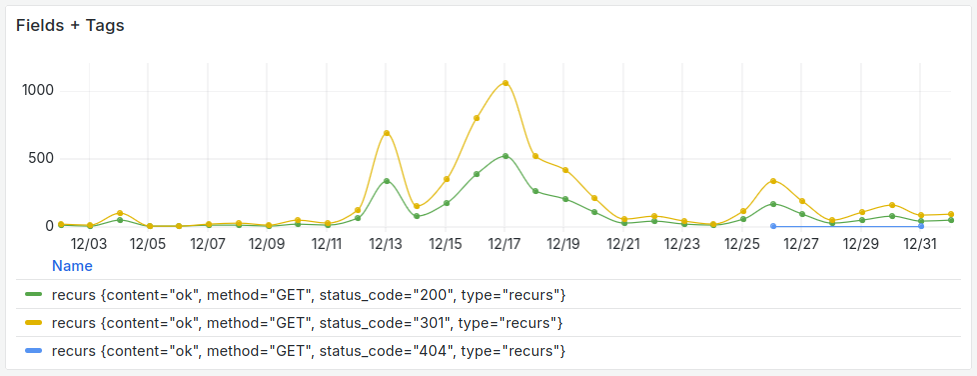
\includegraphics[width=\textwidth]{figures/most-accessed-resource}}
    \captionsetup{justification=centering}
    \caption[Representació del recurs més accedit durant el desembre del 2023.]{Representació del recurs més accedit durant el desembre del 2023. (\textbf{Font}: Elaboració pròpia.)}\label{fig:most-accessed-resource}
\end{figure}

\begin{itemize}
    \item Gràcies al fet que les entrades a la base de dades contenen els camps més rellevants, la classificació per cada paràmetre la realitza \textit{Grafana} automàticament.
    \item Com a conseqüència, per cada combinació del tipus de contingut (\textit{content}), mètode \gls{HTTP} emprat (\textit{method}) i resposta de la petició (\textit{status\_code}) que accedeixin a aquest recurs tindran el seu seguiment.
    \item Podem veure com sempre el contingut del registre d'accés és correcte (content = “ok”) i el mètode utilitzat és el GET.

    La resposta de la petició varia entre un \texttt{200} (succés) o un \texttt{301} (indica que el contingut és a una altra ubicació i et redirigeix)
\end{itemize}

\clearpage
\subsection{Accessos amb el seu contingut alterat}\label{subsec:content-altered-acces}

\textbf{Definició}

\begin{itemize}
    \item Donat un espai de temps, volem consultar quants accessos s'han produït amb malformacions al seu contingut.

    \begin{itemize}
        \item Les malformacions del contingut del accesos, tal i com vam veure a l'apartat de filtratge dels logs (vegeu~\ref{subsec:log-filter}), corresponen a registres que difereixen molt respecte el format general.
        \item Durant l'etapa d'anàlisi i emmagatzemmatge dels logs, vam marcar aquells sospitosos amb una etiqueta.
        Concretament, amb content = “diferent”.
    \end{itemize}

    \item També volem esbrinar com ha sigut la seva evolució al llarg del temps, a més dels paràmetres que s'utilitzen.
\end{itemize}

\noindent \\
\textbf{Anàlisi}

\begin{itemize}
    \item Treballarem sobre l'eina d'observabilitat Grafana, analitzant aquells accessos a recursos que tinguin alteracions en el seu contingut.
\end{itemize}

\noindent \\
\textbf{Representació}

\begin{itemize}
    \item Per fer la representació de les dades escollirem una sèrie temporal.
    \item Seleccionarem una gràfica de tipus Time Series i afegirem a la part inferior la següent cerca.
    Concretament, estem cercant a \textit{InfluxDB}:

    \begin{itemize}
        \item Període del 2023.
        \item Accessos que siguin recursos i el seu contingut sigui diferent.
        \item Comptem els accessos cada trenta dies.
        \item La cerca que utilitzarem és la següent:
    \end{itemize}
\end{itemize}

\noindent
\begin{verbatim}
from(bucket: "upcommons")
  |> range(start: 2023-01-01T00:00:00Z, stop: 2023-12-31T00:00:00Z)
  |> filter(fn: (r) => r["_measurement"] == "tfg")
  |> filter(fn: (r) => r["_field"] == "log")
  |> filter(fn: (r) => r["type"] == "recurs")
  |> filter(fn: (r) => r["content"] == "diferent")
  |> aggregateWindow(every: 30d, fn: count, createEmpty: false)
  |> yield(name: "count")
\end{verbatim}

\clearpage

\noindent \\
\textbf{Resultat}

\begin{figure}[htbp]
    \centerline{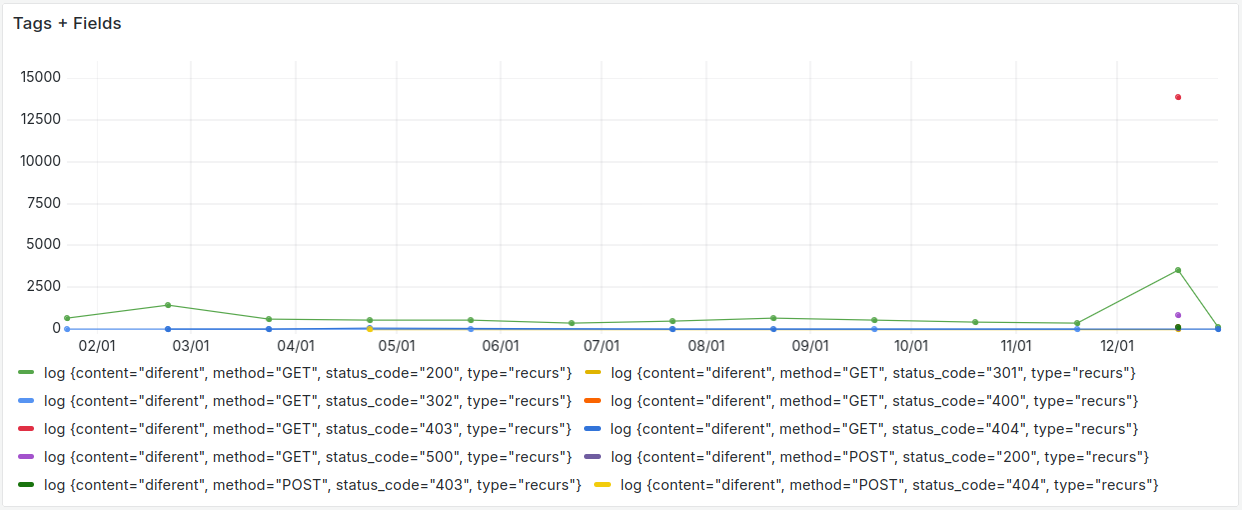
\includegraphics[width=\textwidth]{figures/possible-attacks}}
    \captionsetup{justification=centering}
    \caption[Representació del accessos amb el seu contingut alterat del 2023.]{Representació del accessos amb el seu contingut alterat del 2023. (\textbf{Font}: Elaboració pròpia.)}\label{fig:log-altered}
\end{figure}

\begin{itemize}
    \item Aquest seria el recompte d'accessos a recursos amb el contingut alterat durant l'any 2023, separats per mètode i codi d'estat.
    \item Vora finals d'any, podem observar com hi ha un pic de peticions que no és gens habitual.
    Concretament són peticions GET que retornen un 403.
    \item El codi d'estat 403 del protocol \gls{HTTP} que no estat autoritzat per realitzar aquesta petició.
    \item Explorant una mica més, obtenim que aquest pic correspon a una llarga sèrie de peticions que va augmentar considerablement a partir de les 10:30 h de l'11 de novembre del 2023 i hauria acabat quinze minuts després.
    \clearpage
    \begin{figure}[htbp]
        \centerline{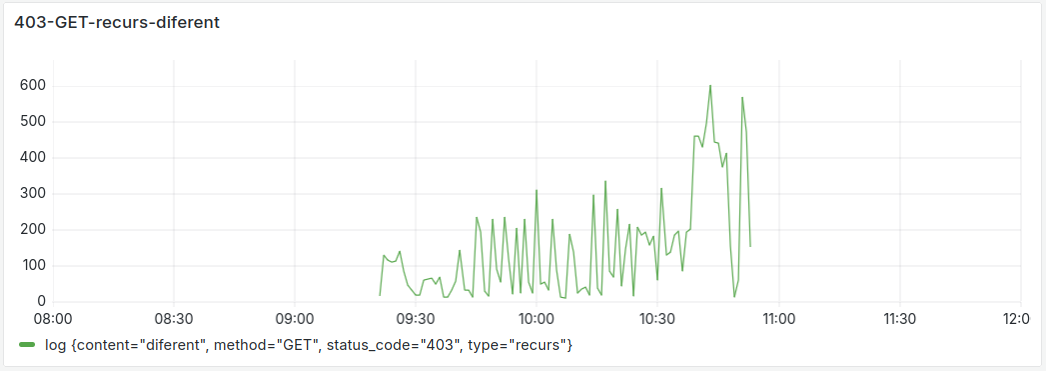
\includegraphics[width=\textwidth]{figures/possible-attacks-403}}
        \captionsetup{justification=centering}
        \caption[Pic de peticions del tipus \texttt{GET} que retornen un codi \texttt{403}.]{Pic de peticions del tipus \texttt{GET} que retornen un codi \texttt{403}. (\textbf{Font}: Elaboració pròpia.)}\label{fig:possible-attacks}
    \end{figure}
    \item Per consultar el contingut d'aquestes peticions ens redirigim a \textit{InfluxDB} i consultem les hores i els paràmetres prèviament determinats.
    \item El patró que segueix és consultar un recurs i afegir paràmetres d'\gls{HTTP} amb valors maliciosos.
    Els més habituals que s'han utilitzat són filter i range.
    La majoria d'aquests registres intenten executar un sleep.
    \item Un exemple, la comparació de dues comandes que retornen el mateix resultat sempre és certa (en vermell), i s'intenta executar un sleep per endarrerir la resposta certs segons. \\
    \begin{figure}[htbp]
        \centerline{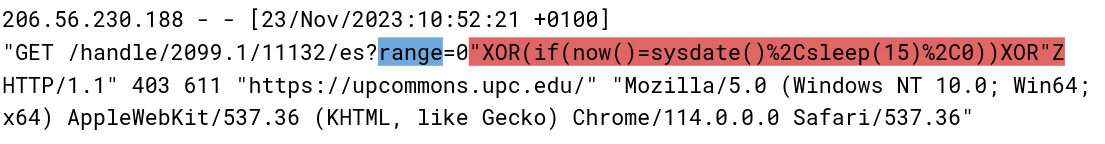
\includegraphics[width=\textwidth]{figures/log-attack}}
        \captionsetup{justification=centering}
        \caption[Exemple d'un intent d'atac a través d'un accés a un recurs.]{Exemple d'un intent d'atac a través d'un accés a un recurs. (\textbf{Font}: UPCommons.)}\label{fig:most-log-attack}
    \end{figure}
\end{itemize}

\clearpage

\subsection{Condicions d’accés dels accessos a recursos de l’EPSEVG}\label{subsec:acces-conditions}

\textbf{Definició}

\begin{itemize}
    \item Donat un període de temps, volem saber quines són les condicions d’accés dels recursos de l’EPSEVG consultats.
    \item Volem analitzar els accessos depenent si són d’accés obert, restringits per l’usuari, per acord de confidencialitat, restringit a la comunitat universitària, etcètera.
\end{itemize}

\noindent \\
\textbf{Anàlisi}

\begin{itemize}
    \item Per obtenir aquestes dades treballarem tant amb la base de dades dels \textit{\gls{log}s} \textit{InluxDB} com amb les metadades, a \textit{MongoDB} .
    \item Per començar, consultem tots els accessos a recursos durant el període de temps determinat.
    En el nostre cas escollim el dia 2023/12/01.
    \item Per cada accés, consultem la base de dades per obtenir el document de metadades relacionat.
    En cas d’obtenir resultat, consultem l’etiqueta \textit{dc.audience.mediator} que ens indica el centre docent relacionat amb el recurs.
    \item Podem obtenir aquest valor pels treballs finals de grau, exàmens, materials docents i vídeos, i d’altres tipologies de manera puntual.
    \item Seguidament, extraiem el valor de l’etiqueta \textit{dc.rights.access}, que conté la informació sobre les condicions d’accés d’aquell recurs.
    \item Agrupant l’identificador del recurs, la condició d’accés i la data i hora de la consulta, afegim aquesta informació a una nova taula a \textit{InfluxDB} anomenada \textit{epsevg-rights}.

\end{itemize}

\clearpage

\noindent \\
\textbf{Representació}

\begin{itemize}
    \item Per fer la representació de les dades escollirem una sèrie temporal.
    \item Seleccionarem una gràfica de tipus Time Series i afegirem a la part inferior la següent cerca.
    Concretament, estem cercant a InfluxDB:
    \begin{itemize}
        \item Període del 2023/12/01.
        \item Obtenim tota la informació dels accessos de la taula \textit{epsevg-rights}.
        \item Comptem els accessos cada hora.
        \item La cerca que utilitzarem és la següent:
    \end{itemize}
\end{itemize}

\noindent
\begin{verbatim}
from(bucket: "upcommons")
  |> range(start: 2023-12-01T00:00:00Z, stop: 2023-12-02T00:00:00Z)
  |> filter(fn: (r) => r["_measurement"] == "epsevg-rights")
  |> filter(fn: (r) => r["_field"] == "recurs")
  |> aggregateWindow(every: 1h, fn: count, createEmpty: false)
  |> yield(name: "count")
\end{verbatim}

\clearpage

\noindent \\
\textbf{Resultat}

\begin{figure}[htbp]
    \centerline{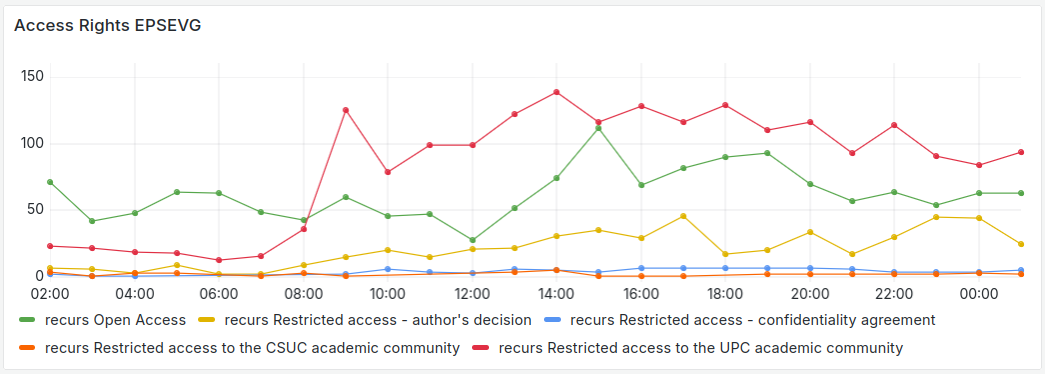
\includegraphics[width=\textwidth]{figures/access-rights-epsevg}}
    \captionsetup{justification=centering}
    \caption[Condicions d'accés dels accessos a recursos de l'EPSEVG el dia 2023/12/01.]{Condicions d'accés dels accessos a recursos de l'EPSEVG el dia 2023/12/01. (\textbf{Font}: Elaboració pròpia.)}\label{fig:log-altered}
\end{figure}

\begin{itemize}
    \item Les diferents condicions d’accés d’aquest període per accessos a recursos són:
    \begin{itemize}
        \item Vermell: recurs restringit a la comunitat acadèmica de la UPC.
        \item Verd: recurs d’accés obert.
        \item Groc: recurs restringit per decisió de l’autor.
        \item Blau: recurs restringit per acord de confidencialitat
        \item Taronja: recurs restringit a la comunitat acadèmica del CSUC (Consorci de Serveis Universitaris de Catalunya)
    \end{itemize}

    \item Les condicions d’accés més habituals són aquelles on més usuaris poden accedir.
    Aquest són l’accés obert i l’accés restringit a la comunitat acadèmica de la UPC .
    \item Cal remarcar que tots els exàmens són restringits a la comunitat acadèmica de la UPC .
    \item Els menys accedits són aquells d’accés restringit a un públic (a vegades nul) petit, sigui per acord de confidencialitat sigui per decisió de l’autor.
    \clearpage
    \item Pel cas dels recursos restringits a la comunitat acadèmica del CSUC (al peu de lletra: “Restricted access to UB, UAB, UPC, UPF, UdG, UdL, URV, UOC, BC, UVic, UJI, URL, UIC users”) es tracta d’accessos a llibres bastant antics.
    \item Dos d’ells tracten principis de desenvolupament sostenible (2099.3/36752 i 2099.3/36834), un altre d’ergonomia (2099.3/36854) i el darrer sobre anàlisi d’antenes (2099.3/36797)

\end{itemize}

\chapter{Conclusion}
\chapter{Agraïments}\label{ch:acknowledgments-ca}
    \addcontentsline{toc}{chapter}{\bibname}
    \bibliographystyle{acm}
    \bibliography{main}

\appendix
\chapter{Open Science Toolkit Information Access}\label{ch:ostia}
El repositori principal on es troba el codi emprat per tractar i analitzar les dades d'accés a \gls{UPCommons} s'anomena Open Science Toolkit Information Access (\gls{OSTIA}), i es troba a públicament a \textit{GitHub}: \url{https://github.com/omar-briqa-tfg/OSTIA}, sota una llicència MIT.

\noindent \\
En aquest s'hi ha desenvolupat les eines necessàries per a la realització del projecte.
Es tracta d'un repositori basat en el sistema de control de versions \textit{\gls{git}}.

\noindent \\
La mecànica de treball sobre aquest tipus de repositoris és la tradicional.
Per cada nova característica que es vulgui afegir al codi font de l'eina, es crea una nova branca.
Tot el procés de desenvolupament es fa sobre aquesta, deixant la branca principal pel codi acabat.

\noindent \\
Per no divergir gaire amb la branca principal, un cop s'acaba la característica que es vol implementar, es disposa a fer la fusió.
Aquest procés se sol fer mitjançant una petició (al context de git, \textit{Pull Request}), ja que com a bona pràctica, la branca principal està protegida per tal d'evitar a tot preu la introducció d'errors, \textit{bugs}, etc.

\noindent \\
Aquesta petició per afegir el nou codi habitualment és revisada per altres membres de l'equip de desenvolupadors, els contribuïdors a l'eina, responsables\dots

\noindent \\
En el nostre cas, la feina ha estat feta individualment, per tant, no tenim aquests segons punts de vista.
Malgrat això, el procés s'ha dut a terme igualment per dos motius:

\begin{itemize}
    \item mantenir un històric de canvis.
    \item modularitat en el desenvolupament.
\end{itemize}{}

\clearpage

\section*{Estructura}\label{sec:ostia-structure}

\noindent
Dividirem l'estructura del repositori de codi en dues parts, encara que convisquin:
\begin{itemize}
    \item Codi relacionat amb el correcte funcionament del mateix repositori.
    \item Codi relacionat amb el processament i l'anàlisi de les dades d'accés a \gls{UPCommons}
\end{itemize}

\noindent \\
La primera part està estructurada de la següent manera:

\begin{verbatim}
    - .github/workflows
    - LICENSE
    - README.md
    - Makefile
    - Pipfile
    - pre-commit-config.yaml
\end{verbatim}

\noindent \\
El propòsit individual és:

\begin{itemize}
    \item \texttt{.github/workflow}: Directori on s'inclouen tots els arxius que defineixen els \textit{\gls{GitHub}} \textit{workflows}.
    Parlem d'accions que s'executen puntualment, com per exemple, després d'afegir codi a la branca principal, durant el procés de \textit{Pull Request}, etc.
    \item \texttt{LICENSE}: llicència sota la qual es desenvolupa el programari.
    \item \texttt{README.md}: per norma general, fitxer informatiu principal als repositoris de \textit{\gls{GitHub}}.
    \item \texttt{Makefile}: fitxer d'automatització de comandes.
    L'utilitzarem per generar la documentació, comprimir el codi principal, crear la imatge de \textit{\gls{Docker}}, etc.
    \item \texttt{Pipfile}: fitxer que defineix les dependències (amb la versió específica) necessàries per al funcionament de l'eina.
    \item \texttt{pre-commit-config.yaml}: fitxer de configuració que imposa unes normes que s'han de complir abans d'enviar un \textit{\gls{commit}}.
\end{itemize}

\clearpage

\noindent \\
Per altra banda, tenim la següent estructura:

\begin{verbatim}
    - config
    - doc
    - scripts
    - src
      |-- logs
      |-- metadata
      |-- queries
      |-- dashboards
    - test
\end{verbatim}

\noindent \\
El propòsit de cada directori és:

\begin{itemize}
    \item \texttt{config}: Emmagatzema els diferents fitxers de configuració requerits durant el processament de les dades.
    Tant la base de dades com els diferents \textit{\gls{plugin}s} utilitzats es troben definits aquí. \\
    Vegeu configuració del servidor~\ref{sec:server-configuration}
    \item \texttt{doc}: Documentació del codi.
    Classes, mètodes, comentaris, excepcions, etc.
    Inclou una eina per generar manualment aquesta documentació.
    \item \texttt{scripts}: Conjunt de \textit{scripts} que ajuden a automatitzar certes tasques.
    No formen part del codi principal de l'eina, però sí que en complementen aquesta.
    \item \texttt{src}: Directori principal de codi.
    Es troba el codi font emprat per la realització del projecte.
    Està escrit en Python.
    Consta de:
    \begin{itemize}
        \item \texttt{logs}: processament i emmagatzematge dels \textit{logs}.
        \item \texttt{metadata}: processament i emmagatzematge de les metadades.
        \item \texttt{queries}: anàlisi de les dades.
        \item \texttt{dashboards}: panells de Grafana en format \gls{JSON}.
    \end{itemize}
    \item \texttt{test}: Directori que conté proves del funcionament de l'eina.
\end{itemize}


\chapter{Servidor de treball}\label{ch:server-description}

El procés de desenvolupament s’ha dut a terme emprant un servidor preparat pels directors del projecte, amb les següents característiques:

\begin{itemize}
    \item \textbf{Processador:}
    \begin{itemize}
        \item quatre cores
    \end{itemize}
    \item \textbf{Emmagatzemament:}
    \begin{itemize}
        \item 16 GB de disc de sistema
        \item 256 GB de disc SSD per dades
    \end{itemize}
\end{itemize}

\noindent
Aquest disposa de dos usuaris, \textit{tfe}, per l’ús diari, i un altre, amb privilegis d’administrador, \textit{root}, en cas que es necessitin aquests.
L’accés es realitza a través de l’usuari tfe, utilitzant una connexió \gls{ssh}:

\begin{verbatim}
    $ ssh tfe@ostia.epsevg.upc.edu
\end{verbatim}

\noindent
Les tasques principals realitzades són:

\begin{itemize}
    \item Desenvolupament del codi d’\gls{OSTIA}, utilitzant el sistema de control de versions git.
    \item Anàlisis dels logs d’\gls{UPCommons}, amb registres des del 2006 fins al 2023.
    \item Processament i abocament dels logs a la base de dades InfluxDB, ubicada al mateix servidor.
    \item Descàrrega de totes les metadades del servidor \gls{OAI} sbivdev1.
    \item Anàlisis, processament i abocament de les metadades a una base de dades MongoDB.
    \item Anàlisi quantitativa i qualitatiu del conjunt de les dades, amb el suport l’eina Grafana.
\end{itemize}

\clearpage

\section{Configuració}\label{sec:server-configuration}

Els principals serveis utilitzats durant la realització del projecte han sigut:

\begin{itemize}
    \item \textbf{InfluxDB}
    \begin{itemize}
        \item Base de dades on hem emmagatzemat els logs.
        \item {
            Incorporem també el \textit{\gls{plugin}} d’InfluxDB anomenat Telegraf.
            Encara que el seu ús no és imperatiu pels nostres objectius, pot ser útil per recol·lectar dades del sistema.
        }
    \end{itemize}
    \item \textbf{MongoDB}
    \begin{itemize}
        \item Base de dades utilitzada per l’emmagatzematge de les metadades.
        \item El mateix servei no ofereix cap interfície gràfica, així doncs afegim el suport de mongodb-expres.
    \end{itemize}
    \item \textbf{Grafana}
    \begin{itemize}
        \item Principal eina d’observabilitat, emprada tant per l’anàlisi com per la visualització gràfica.
    \end{itemize}
\end{itemize}

\noindent
Per cadascun d’aquests serveis definirem un fitxer de configuració, que configurarà cada contenidor, que en aquest cas, són de tipus \textit{\gls{Docker}}. \\

\noindent
Com disposem de diverses aplicacions, la manera més senzilla és utilitzar el sistema per configurar i executar aplicacions multi-contenidor per antonomàsia, que és \textit{\gls{docker-compose}}. \\

\noindent
Aquest fitxer acostuma a tenir aquesta estructura:

\begin{itemize}
    \item Definició del nom del servei.
    \item Imatge de \textit{\gls{Docker}} que es vol utilitzar.
    \item Els ports, definint el port de la màquina host i el del contenidor.
    \item El fitxer de configuració del servei.
    \item La xarxa interna del servei de \textit{\gls{Docker}} que adoptarà el servei.
    \item Altres opcions.
\end{itemize}

\clearpage

\noindent
A l'exemple següent es troba la configuració específica per la base de dades InfluxDB.

\begin{figure}[htbp]
    \centerline{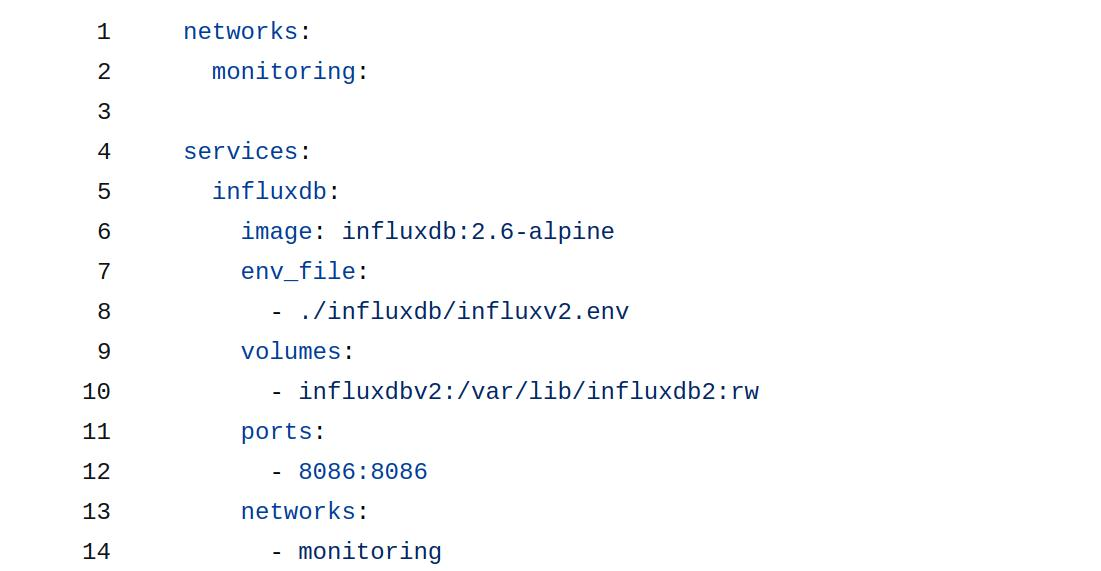
\includegraphics[width=\textwidth]{figures/docker-compose-influxdb}}
    \captionsetup{justification=centering}
    \caption{Configuració del servei d'InfluxDB.}\label{fig:docker-compose-influxdb}
    \source{Repositori de codi del projecte.}
\end{figure}

\begin{tcolorbox}[colback=blue!5!white, colframe=blue!75!black, title=Fitxers de configuració]
    Habitualment aquests fitxers solen incloure credencials privades d'aquests serveis.
    Com a bona pràctica, afegeix el sufix \textit{.env} al fitxer i no el pugis a Github, omitin-lo mitjançant el fitxer \textit{.\gls{gitignore}}.
\end{tcolorbox}
\vspace{1em}

\noindent
Un cop definits tots els serveis, es procedeix amb la instal·lació.
La comanda següent, descarrega les imatges de \textit{\gls{Docker}} en cas que aquestes no estiguin presents al sistema,
crea les xarxes virtuals pels contenidors i finalment, configura els serveis.

\begin{verbatim}
    $ docker compose up -d
\end{verbatim}

\begin{tcolorbox}[colback=red!5!white, colframe=red!75!black, title=Atenció]
    Aquesta comanda s'ha d'executar en el mateix directori on es troba el fitxer \textit{\gls{docker-compose}}.
\end{tcolorbox}

\clearpage

\section{Accés als serveis}\label{sec:server-access}

\noindent
Per accedir als diferents serveis que es troben al servidor, utilitzarem un túnel ssh~\cite{tunel-ssh}.
Aquest consisteix en xifrar tota comunicació entre client i servidor. \\

\noindent
Per exemple, el contingut de la interfície gràfica de Grafana, accessible a través del port tres mil del servidor,
serà accessible pel port tres mil de la màquina \textit{host} amb els següents passos:

\begin{verbatim}
    $ ssh -N -L localhost:3000:ostia.epsevg.upc.edu:3000 \
        tfe@ostia.epsevg.upc.edu
\end{verbatim}
\begin{verbatim}
    $ open https://localhost:3000
\end{verbatim}
\chapter{Instal·lació de software}\label{ch:software-installation}

\section*{\gls{Docker}}\label{sec:docker-installation}

\begin{tcolorbox}[colback=blue!5!white, colframe=blue!75!black, title=sudo]
    La comanda \textit{sudo} és prescindible en cas d'estar utilitzant un usuari amb permisos d'administrador, com en el nostre cas, l'usuari \textit{root}.
\end{tcolorbox}

\noindent \\
Actualitzem la llista de paquets.
\begin{verbatim}
$ sudo apt-get update
\end{verbatim}

\noindent \\
Insta·lem les dependències requerides per \textit{\gls{Docker}}.
\begin{verbatim}
$ sudo apt-get install -y apt-transport-https ca-certificates \
    curl software-properties-common
\end{verbatim}

\noindent \\
Descarreguem, convertim a format binari i emmagatzemem la clau GPG oficial de \textit{\gls{Docker}}
\begin{verbatim}
$ curl -fsSL https://download.docker.com/linux/debian/gpg \
    | sudo gpg --dearmor \
    -o /usr/share/keyrings/docker-archive-keyring.gpg
\end{verbatim}

\noindent \\
Afegim a la llista de repositoris, el repositori de \textit{\gls{Docker}} corresponent a la nostra distribució.
\begin{verbatim}
$ echo "deb [arch=amd64 \
    signed-by\rightthreetimes=/usr/share/keyrings/docker-archive-keyring.gpg] \
    https://download.docker.com/linux/debian $(lsb_release -cs) stable" \
    | sudo tee /etc/apt/sources.list.d/docker.list > /dev/null\bullet
\end{verbatim}

\clearpage

\noindent \\
Instal·lem els paquets de \textit{\gls{Docker}}.
\begin{verbatim}
$ sudo apt install docker-ce docker-ce-cli containerd.io
\end{verbatim}

\noindent \\
Iniciem el servei.
\begin{verbatim}
$ sudo systemctl start docker
\end{verbatim}

\noindent \\
Habilitem que el servei s'inicii automàticament cada vegada que es reinicia el sistema.
\begin{verbatim}
$ sudo systemctl enable docker
\end{verbatim}

\chapter{Configuració de \textit{Grafana}}\label{ch:grafana-config}

Grafana és la nostra eina principal observabilitat, i que ens permetrà visualitzar els nostres casos d’ús.
Per poder fer-la servir l’haurem de configurar per tal que aquesta consumeixi de la nostra base de dades principal, \textit{InfluxDB} .

\noindent \\
Malauradament, aquesta eina no incorpora suport directe amb \textit{MongoDB}, per tant, l’anàlisi general sobre les metadades s’haurà de fer per separat. \\ \\

\section*{Connexió amb InfluxDB}\label{sec:influxdb-grafana-connection}

\noindent
Per afegir una font de dades a Grafana a les darreres versions es realitza a través de la pestanya \textit{Connections}.
Seguidament,  escollirem \textit{InfluxDB} a l'apartat de ``Add new connections'', on podrem escollir diferents fonts de dades (\textit{data sources}). \\

\noindent
\begin{tcolorbox}[colback=blue!5!white, colframe=blue!75!black, title=Llenguatge de cerca]
    InfluxDB suporta diferents llenguatges per realitzar les seves consultes.
    Però, el recomanable i més actualitzat és \textit{Flux}.
    Això és important degut que la configuració varia en funció del llenguatge escollit.
\end{tcolorbox}

\noindent \\
Escollirem el llenguatge Flux.
Les altres opcions són \textit{InfluxQL} i \textit{SQL}, no les farem servir.
Ara passem a la configuració.

\clearpage

\noindent \\
Per l’apartat d’HTTP definirem l’\gls{URL} del servei.
Com el servei \gls{DNS} de la xarxa de Docker ja resol el servei pel seu nom, l’hem de definir per \textbf{influxdb}.
Utilitzar \textbf{localhost} podria errar durant l’intent de connexió.

\begin{figure}[htbp]
    \centerline{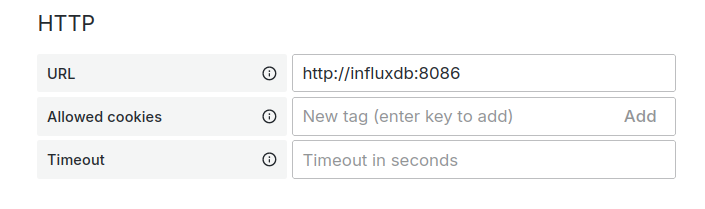
\includegraphics[width=\textwidth]{figures/grafana-influxdb-http}}
    \captionsetup{justification=centering}
    \caption[Configuració \gls{HTTP} d'\textit{InfluxDB} a \textit{Grafana}.]{Configuració \gls{HTTP} d'\textit{InfluxDB} a \textit{Grafana}. (\textbf{Font}: Aplicatiu \textit{Grafana} del servidor de treball.)}\label{fig:grafana-influxdb-http}
\end{figure}

\noindent \\
Pel que fa a l’autenticació, afegirem les nostres credencials d’\textbf{InfluxDB}.
La paraula clau \textbf{configured} indica que la contrasenya ja ha sigut introduïda, i no que aquesta sigui ``configured''.

\begin{figure}[htbp]
    \centerline{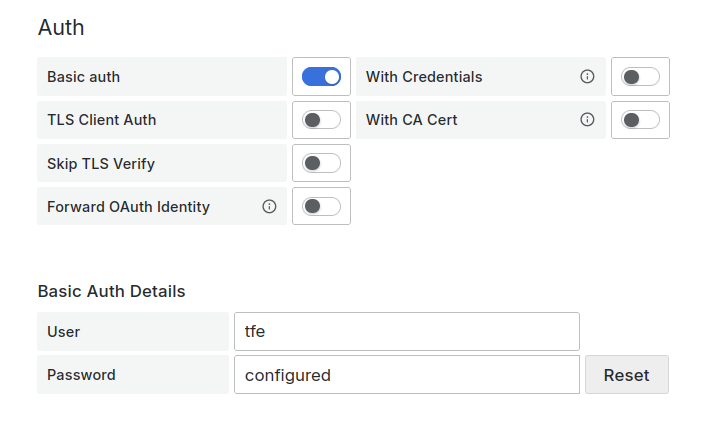
\includegraphics[width=\textwidth]{figures/grafana-influxdb-auth}}
    \captionsetup{justification=centering}
    \caption[Configuració d'autenticació d'\textit{InfluxDB} a \textit{Grafana}.]{Configuració d'autenticació d'\textit{InfluxDB} a \textit{Grafana}. (\textbf{Font}: Aplicatiu \textit{Grafana} del servidor de treball.)}\label{fig:grafana-influxdb-auth}
\end{figure}

\clearpage

\noindent
Finalment, completarem els detalls d’InfluxDB, que són l’organització i els altres paràmetres definits durant la configuració d’\textit{InfluxDB}.
El \textit{token} és el clau que utilitzarem com autenticació a l’hora de realització de consultes.

\noindent \\
Aquest \textit{token} es genera a la interfície de la base de dades.
Hem de tenir en compte d’assignar els permisos de lectura/escriptura correctes.
D’altra manera, no podrem realitzar les consultes pertinents.

\begin{figure}[htbp]
    \centerline{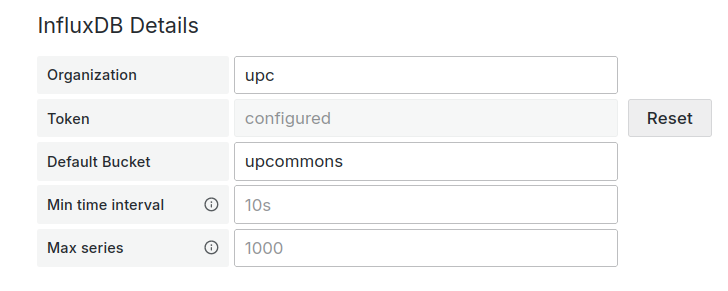
\includegraphics[width=\textwidth]{figures/grafana-influxdb-details}}
    \captionsetup{justification=centering}
    \caption[Configuració dels detalls d'\textit{InfluxDB} a \textit{Grafana}.]{Configuració dels detalls d'\textit{InfluxDB} a \textit{Grafana}. (\textbf{Font}: Aplicatiu \textit{Grafana} del servidor de treball.)}\label{fig:grafana-influxdb-details}
\end{figure}

\clearpage

\section*{Creació de \textit{dashboards}}\label{sec:grafana-dashboards}

\noindent
Afegir panells de visualització és una tasca senzilla un cop tens definit el teu cas d'ús, les dades que vols tractar i quin tipus de representació visual vols realitzar.

\noindent \\
Els passos són:
\begin{center}
    Dashboards \(\rightarrow\) New Dashboard \(\rightarrow\) Add Visualization
\end{center}

\noindent
Has d’escollir la font de dades.
Apareixerà l0InfluxdDB que prèviament s’ha configurat.
Seguidament emeregeixen tres finestres principals, adaptables en mida.

\noindent \\
La finestra central mostrarà la representació de les dades.
A la part inferior, hi ha un editor on es pot introduir la cerca a \textit{InfluxDB} .
Un cop introduïda, s'emmagatzema i s'executa automàticament.

\begin{figure}[htbp]
    \centerline{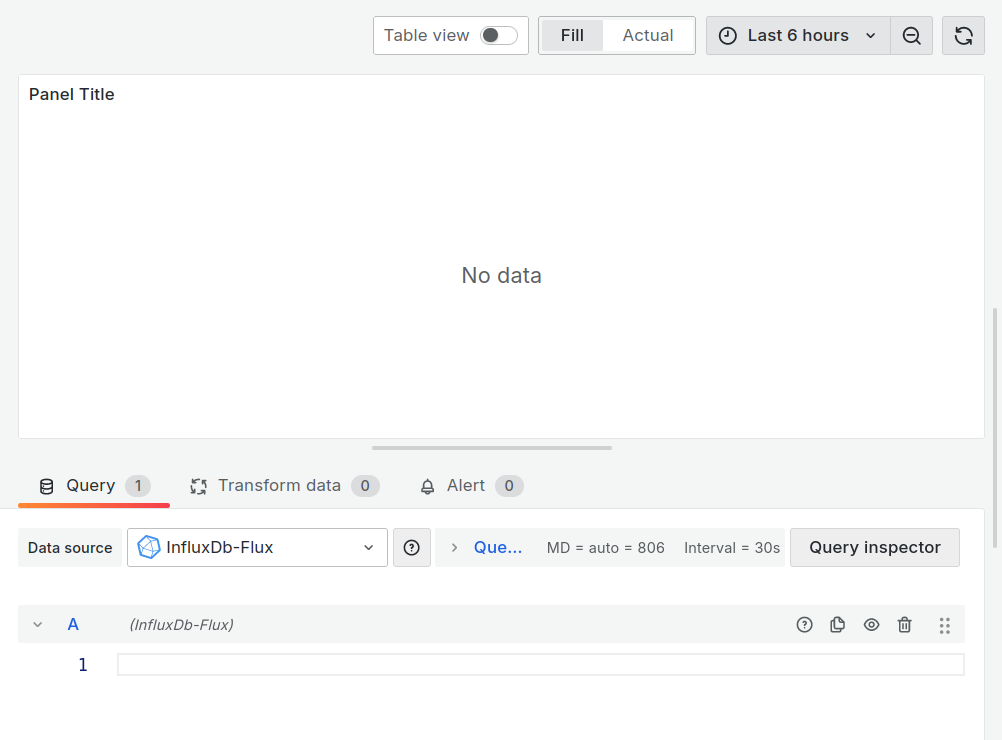
\includegraphics[width=\textwidth]{figures/grafana-main-panel}}
    \captionsetup{justification=centering}
    \caption[Finestra principal d'un panell de \textit{Grafana}.]{Finestra principal d'un panell de \textit{Grafana}. (\textbf{Font}: Aplicatiu \textit{Grafana} del servidor de treball.)}\label{fig:grafana-main-panel}
\end{figure}

\clearpage

\noindent
A la part dreta es troba una finestra per personalitzar el panell, tant colors, llegenda, estils, etcètera.
L’opció més important es troba a la part superior, on pots definir el tipus de representació: sèrie temporal, diagrama de barres, intensitat de colors, histogrames, i infinites més opcions.
Sempre que s’adaptin les dades per cada tipus de representació, endavant!

\begin{figure}[h]
    \centering
    \begin{subfigure}{0.45\textwidth}
        \centering
        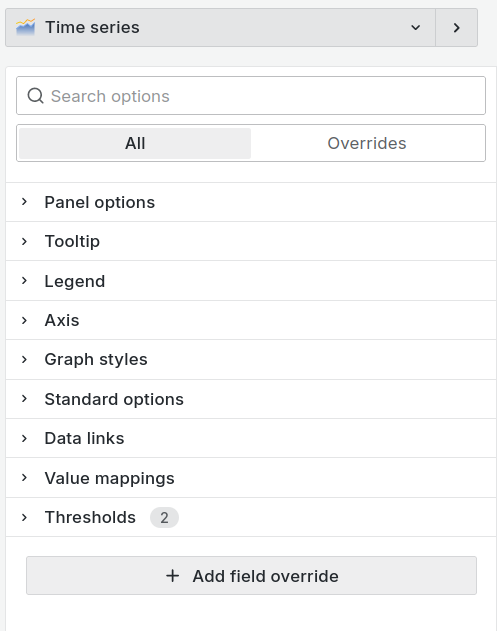
\includegraphics[width=\linewidth]{figures/grafana-panel-customization}
        \label{fig:figure1}
    \end{subfigure}
    \hspace{0.05\textwidth}
    \begin{subfigure}{0.45\textwidth}
        \centering
        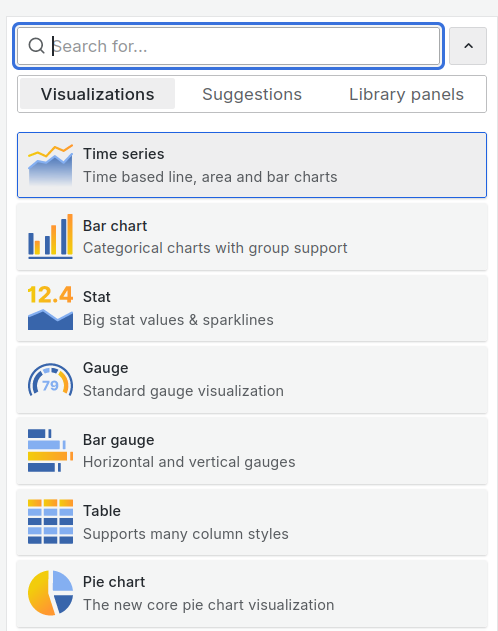
\includegraphics[width=\linewidth]{figures/grafana-panel-visualization-type}
        \label{fig:figure2}
    \end{subfigure}
    \captionsetup{justification=centering}
    \caption[Esquerra: Personalització dels panells de \textit{Grafana}.Esquerra: Personalització dels panells de \textit{Grafana}. \\ Dreta: Tipus de visualització pels panells de \textit{Grafana}. Dreta: Tipus de visualització pels panells de \textit{Grafana}.]{Esquerra: Personalització dels panells de \textit{Grafana}. \\ Dreta: Tipus de visualització pels panells de \textit{Grafana}. (\textbf{Font}: Aplicatiu \textit{Grafana} del servidor de treball.)}
    \label{fig:grafana-panel-visualization}
\end{figure}

\chapter{Resultat de l'abocament dels logs}\label{ch:log-push-results}


\end{document}